\appendix
\chapter{Appendix}

\section{CTM3 specifications}\label{app:CTM3}
\begin{table}[ht]
\centering
\begin{tabular}{|l|l|}
\hline
Value & PLAND-type   \\ \hline
0     & Ocean        \\ \hline
1     & Land         \\ \hline
2     & Lake         \\ \hline
3     & Small island \\ \hline
4     & Ice shelf    \\ \hline
\end{tabular}
\caption{\texttt{PLAND} is based on the \texttt{landsea.nc}-file from \protect\url{/work/projects/cicero/ctm_input/Indata_CTM3}}
\label{tab:PLAND}
\end{table}

\begin{figure}[ht]
    \centering
    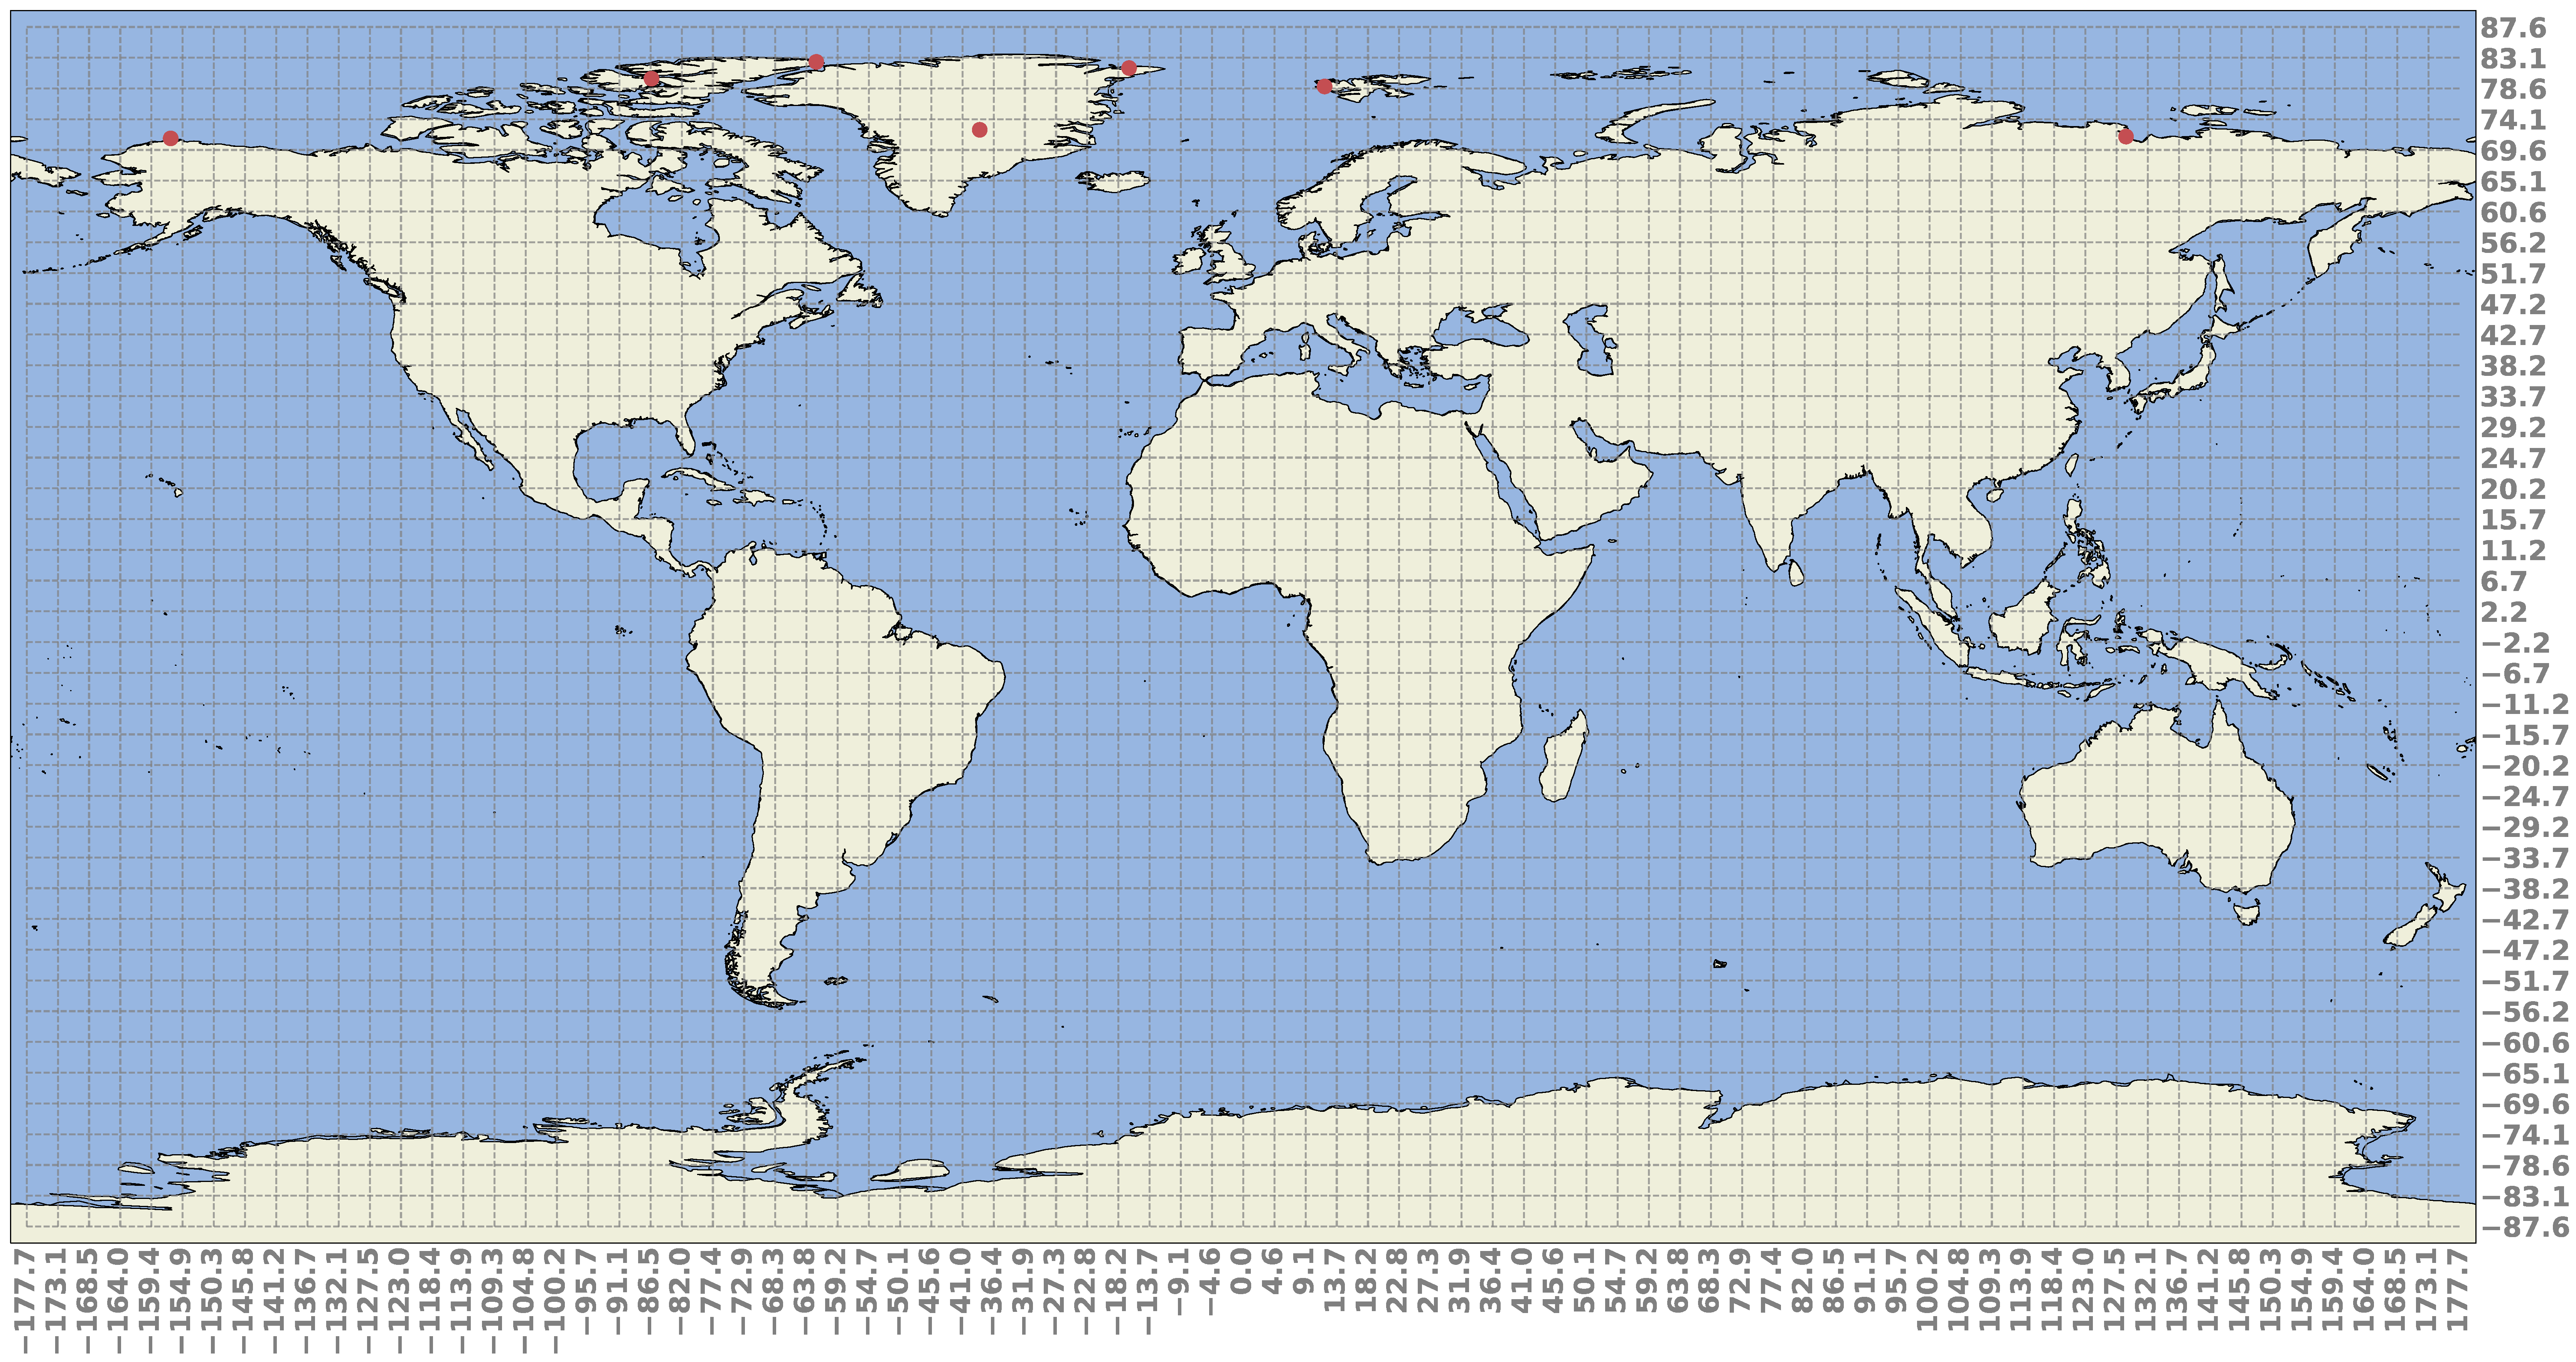
\includegraphics[width = \linewidth]{Appendix/images/resolution_map.pdf}
    \caption{Illustration of the grid coverage in the Oslo CTM3 globally at \texttt{HFOUR} $=$ 4.5$^o$x4.5$^o$ resolution. The red dots are the stations that were used for observational data}
    \label{fig:res_map_global}
\end{figure}

\clearpage
\section{Supporting Figures From Litterature}\label{app:supp_fig}

\begin{figure}
    \centering
    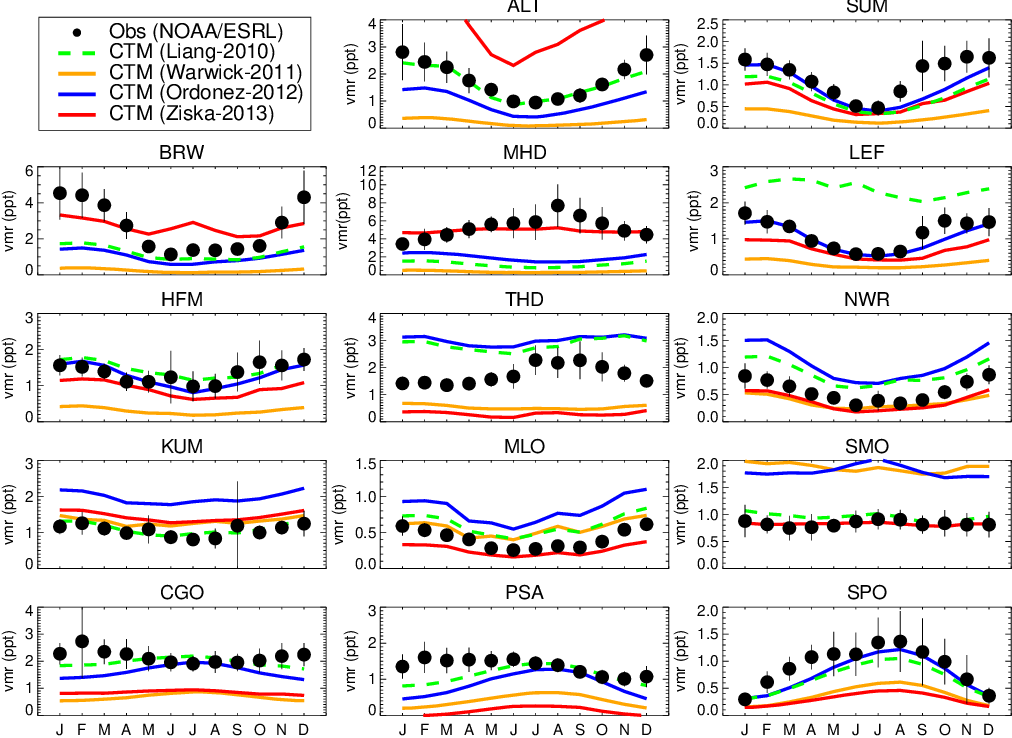
\includegraphics[width =0.7\linewidth]{Appendix/images/Hossaini2013_fig5_bromoform.png}
    \caption{Comparison of monthly mean mixing ratio (ppt) of $\chem{CHBr_3}$ output from \cite{Liang2010}, \cite{ziska}, warwick 2011, ordonez 2012}
    \label{fig:Hosaini_fig5}
\end{figure}

\begin{figure}
    \centering
    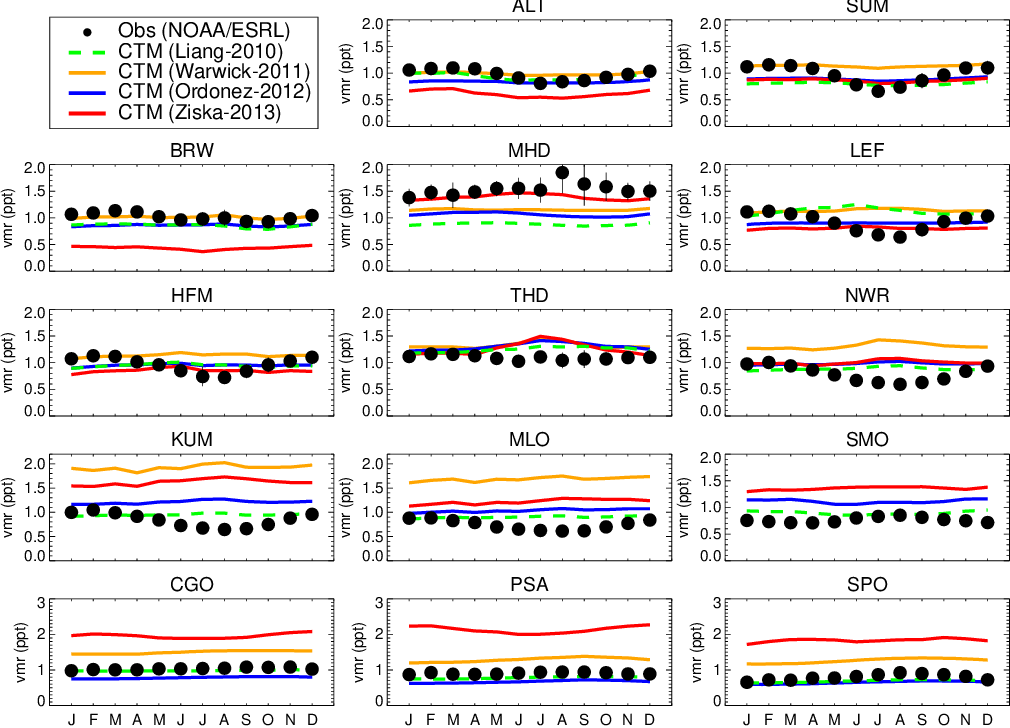
\includegraphics[width =0.9\linewidth]{Appendix/images/Hossaini2013_fig6_ch2br2.png}
    \caption{Comparison of monthly mean mixing ratio (ppt) of $\chem{CH_2Br_2}$ output from \cite{Liang2010}, \cite{ziska}, \cite{Warwick2006} and \cite{Ordonez2012}. The figure is adapted from \cite{Hossaini2013}}
    \label{fig:Hosaini_fig6}
\end{figure}


\begin{figure}[h]
    \centering
    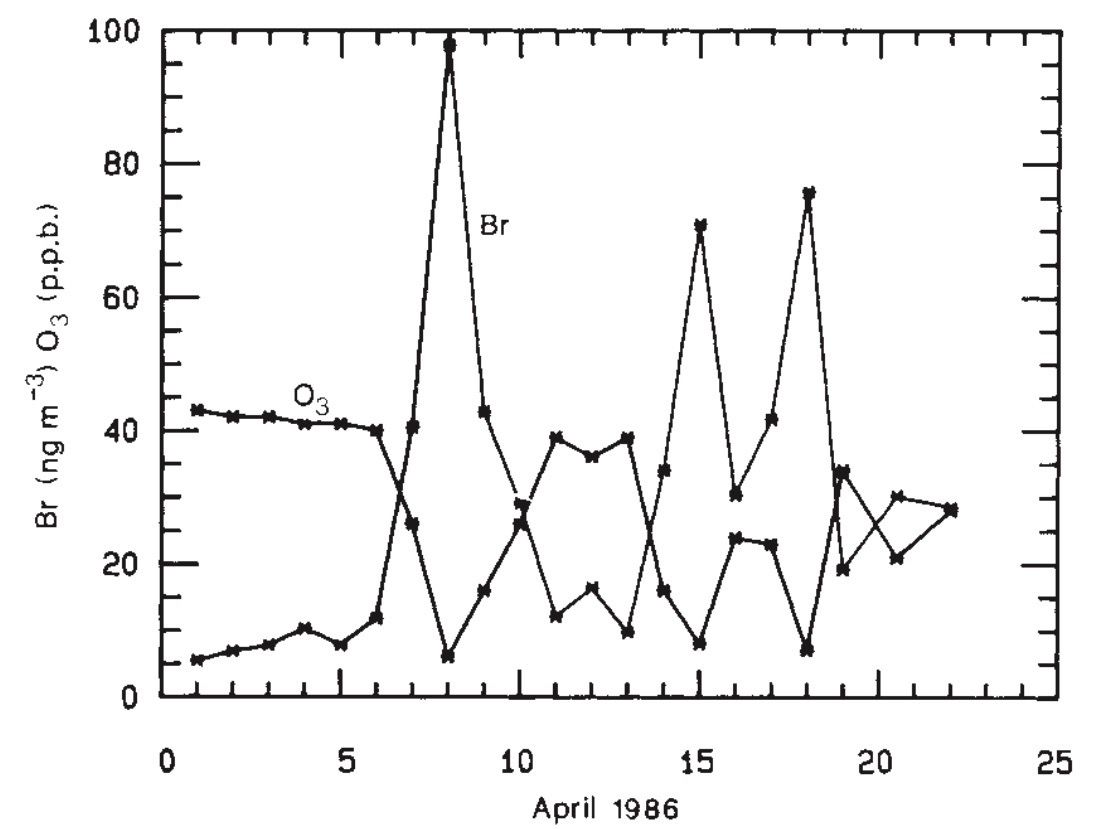
\includegraphics[width =0.8\linewidth]{Appendix/images/Barrie_1988.jpeg}
    \caption{Daily mean ground level $\chem{O_3}$ and filterable \chem{Br} (\chem{f-Br}) concentrations at Alert, Canada in April 1986. The figure is adapted from \cite{barrie}}
    \label{fig:Barrie_1988}
\end{figure}

\begin{figure}
    \centering
    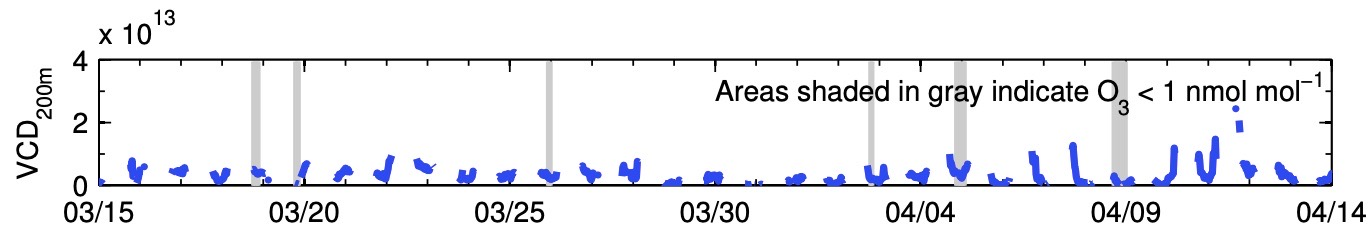
\includegraphics[width =0.9\linewidth]{Appendix/images/Peterson_2015.jpeg}
    \caption{\acrlong{vcd} ($molecules cm^{-2}$) of \chem{BrO} in the lowermost 200 m of the troposphere observed at Barrow, Alaska in 2012. The figure is adapted from \cite{Peterson2015}.}
    \label{fig:Peterson_2015}
\end{figure}

\cleardoublepage

\chapter{EBAS and NOAA Data}\label{app:ebas_noaa_data}


\section{Station Data}

Some key information about the station data obtained from ebas (\cite{EBAS}) is listed in Table \ref{tab:ebas_noaa_data_taken}. The chloride- and bromide- data were compared to the \chem{HBr}- and \chem{HCl}-concentration modelled as the measurements refers to filterable \chem{HBr} (the sum of particulate bromide and \chem{HBr} in the gas-phase). According to \cite{barrie}, these measurements contain about 50-93\% \chem{HBr}. 

\begin{table}[ht]
\centering
\resizebox{14cm}{!}{%
\begin{tabular}{|lllllll|}
\hline
\textbf{Station}  & \textbf{Variable}  & \textbf{Temporal res.} & \textbf{Timzone} & \textbf{Unit}  & \textbf{Instrument type} & \textbf{Year} \\ \hline
Alert            & $\chem{O_3}$ & 1h           & UTC              & $\mu$gm$^{-3}$  & uv\_abs                  & 2001               \\
Alert            & \chem{Cl}    & 1w           & UTC              & $\mu$gm$^{-3}$  & high\_vol\_sampler       & 2001, 2013         \\
Alert            & \chem{Br}    & 1w           & UTC              & $\mu$gm$^{-3}$  & high\_vol\_sampler       & 2001, 2013         \\
Barrow           & $\chem{O_3}$ & 1h           & UTC              & nmol/mol        & uv\_abs                  & 2001, 2013, 2018   \\
Eureka           & $\chem{O_3}$ & 1h           & UTC              & nmol/mol        & uv\_abs                  & 2018               \\
Summit           & $\chem{O_3}$ & 1h           & UTC              & nmol/mol        & uv\_abs                  & 2001, 2013, 2018   \\
Tiksi            & $\chem{O_3}$ & 1h           & UTC              & nmol/mol        & uv\_abs                  & 2013, 2018         \\
Villum           & $\chem{O_3}$ & 1h           & UTC              & $\mu$gm$^{-3}$  & uv\_abs                  & 2013               \\
Villum           & \chem{Cl}    & 1w           & UTC              & $\mu$gm$^{-3}$  & filter\_3pack            & 2013, 2017         \\
Villum           & \chem{Br}    & 1w           & UTC              & $\mu$gm$^{-3}$  & filter\_3pack            & 2017               \\
Zeppelin         & $\chem{O_3}$ & 1h           & UTC              & $\mu$gm$^{-3}$  & uv\_abs                  & 2001, 2013, 2018   \\ \hline
\end{tabular}
}
\caption{Key information about data taken from the different stations (\cite{EBAS}). The arithmetic mean value was used from all datasets. The temporal resolution, timezone and unit were given by each dataset. uv\_abs refers to the ultraviolet absorption method (For more information, see e.g. \cite{Galbally2013}). high\_vol\_sampler and filter\_3pack. The years were chosen according to when the model simulations were planned}
\label{tab:ebas_noaa_data_taken}
\end{table}


\section{Ozonosonde Data}

Ozonosonde measurements from Summit, Greenland, was obtained from \cite{NOAA} for the year 2013. The ozonosonde measures ozone by using an Electrochemical Concentration Cell Ozonosonde (For more information, visit \cite{ESRL}).  

\cleardoublepage

\chapter{Running the CTM3}\label{app:running_CTM3}

\section{The Supercomputer}\label{app:supercomputer}

\subsection{The Job File}

The job file is used to set up a run. The job file declares the job name, the input file, the project number and the wall clock limit, i.e. the max running time in the super computer and the number of nodes to use on the supercomputer when running the simulation. Also, it contains the path to the restart files (information about restart files can be found in Section \ref{subsec:restart_files}).

\subsubsection{Abel vs. Saga}

As the Oslo CTM3 was not optimized for Saga, the job file setup at Saga and Abel differed slightly. At Abel, the most efficient setup was the following: 

\begin{lstlisting}
#!/bin/bash
# Script for running on Abel.
# ----------------------------------------------
# Job name (enter your distinct job name):
#SBATCH --job-name=C3RUN_almost_BE
#
# Project (enter your noturn project number):
#SBATCH --account=geofag
#
# Wall clock limit (setting for one year 96:0:0):
#SBATCH --time=0:30:0
#
# Does your job exceed one week, use "--partition=long":
# ####SBATCH --partition=long
#
# Max memory usage:
#SBATCH --mem-per-cpu=3000M
#
# Number of cores:
#SBATCH --ntasks-per-node=16
#
# Number of nodes:
#SBATCH --nodes=1
#
#
## Set up job environment
source /cluster/bin/jobsetup
\end{lstlisting}

The number of nodes had to be different at Saga as it was slowed down by an increased number: 

\begin{lstlisting}
#!/bin/bash
# Script for running on Saga.
# ----------------------------------------------
# Job name (enter your distinct job name):
#SBATCH --job-name=C3RUN_BE_PI_HFOUR_MarchMay_2013
#
# Project (enter your noturn project number):
#SBATCH --account=nn9188k
#
# Wall clock limit (setting for one year 96:0:0):
#SBATCH --time=15:0:0
#
# Does your job exceed one week, use "--partition=long":
# ####SBATCH --partition=long
#
# Max memory usage:
#SBATCH --mem-per-cpu=3000M
#
# Number of cores:
#SBATCH --ntasks=1
#SBATCH --cpus-per-task=8
#
# Number of nodes:
#SBATCH --nodes=1
#
#
## Set up job environment:
#set -o errexit  # Exit the script on any error
set -o nounset  # Treat any unset variables as an error
\end{lstlisting}


\subsection{The Input File}

The input file consists of three parts, one that sets up the meteorological year, start day and end day. The second part lists some of the input file names, including the tracer lists. Information of the tracer list used here can be found in Section \ref{subsubsec:Ltracer_list} and \ref{subsubsec:tracer_list}. The third part covers information about the diagnostics. 

\medskip

In order to save CPU time and avoid conflicts regarding the use of stratospheric methyl bromide ($\chem{CH_3Br}$) as a designated species for $\chem{CHBr_3}$ and $\chem{CH_2Br_2}$ (explained further in Section \ref{sec:oceanic_emissions}), the stratosphere was turned off. How this was performed is explained in Section \ref{app:turning_off_the_stratosphere}.

\medskip

In the Pre-industrial setups are slightly different and explained in Section \ref{app:PI_run}

\section{Emission List - \texttt{Ltracer\_emis\_ceds17\_YEAR\_megan.d}}
\label{subsubsec:Ltracer_list}

The tracer list contains all the emission information that the model needs to be able to run. The emission inventory used in this thesis is the \acrlong{ceds} inventory and the \acrlong{megan}, version 2.10, inventory. 

\medskip

\acrshort{ceds} is a historical emission inventory for anthropogenic aerosol and precursor compounds (\cite{Lund2018}). The historical emissions are only available for the 1750-2014 period, which limits the possibilities for simulations after 2014 in this thesis. 

\medskip

\acrshort{megan} v2.10 is a framework used by the model to estimate biogenic fluxes between terrestrial ecosystems and the atmosphere (\cite{Guenther2012}). 



\section{Tracer List - \texttt{tracer\_list\_no\_stratosphere.d}}\label{subsubsec:tracer_list}

The tracer list contains all the tracers that the model need in the simulation, with names and molecular weights. It contains two parts - one with transported species and one with non-transported species. The total number of transported and non-transported must match the \texttt{NPAR} and \texttt{NOTRPAR} in \texttt{cmn\_size.F90} (see Section \ref{subsubsec:cmn_size}) (\cite{SovdeManual}). 

\medskip

The list \texttt{tracer\_list\_no\_stratosphere.d} was created in order to include some of the stratospheric chemistry components as well as the components mentioned above. The added components were: 

\begin{itemize}
    \item \textbf{Transported}: $\chem{Cl_x}$, $\chem{HCl}$, $\chem{Cl_y}$, $\chem{CH_3Br}$, $\chem{Br_y}$, $\chem{ClO}$, $\chem{Cl_2}$, $\chem{HBr}$, $\chem{BrONO_2}$, $\chem{OHBr}$, $\chem{Br_2}$, $\chem{BrCl}$, $\chem{Cl}$, $\chem{Br}$, $\chem{BrO}$
    \item \textbf{Non-transported}: $\chem{H_2}$
\end{itemize}

The three components $\chem{Cl}$, $\chem{Br}$, $\chem{BrO}$ were moved from non-transported in the \texttt{bromine\_explosion}-branches, in order to have transport for these species. They were left in non-transported in the \texttt{origCTM3\_noStrat}-branches, as the lack of chemistry for those species in the original CTM3-branches led to conflicts (for an overview of the branches, see Section \ref{sec:code_availability}). 




\section{Restart Files}\label{subsec:restart_files}


The restart file is a NetCDF file that contains the tracer distribution and moments for all species in a simulation. For the transported species, it has prefix \texttt{STT}, and \texttt{XSTT} for the non-transported species. The transported species are associated with their moments, which has the prefixes \texttt{SUT}, \texttt{SVT}, \texttt{SWT}, \texttt{SUU}, \texttt{SVV}, \texttt{SWW}, \texttt{SUV}, \texttt{SUW}, \texttt{SVW} (\cite{SovdeManual}). The restart file is used as an initial field for the production run, which requires a spin up, and it is therefore necessary to determine the length of the spin up (in model time) according to the lifetime of the chemical species of interest. 

\medskip

Restart files used in \cite{Falk_2019} was provided by Stefanie (\texttt{ctm3\_restart\_20010101.nc}) and used for my own spin-up. The provided restart file was spun-up over a 10 years transient run starting in 1990. It was necessary to make new restart files, as the code is changed and the stratosphere is turned off, which alters the chemistry. The restart files were thus based on the same emission inventory (MEGAN and CEDS17) except for biomass burning which was taken from CEDS17 instead of GFed. The reason for this is that the GFed files only exist until 2005, and my intent was to run the model in later years as well. 

\medskip


The dry-deposition scheme also differs, where I have used the old dry-deposition scheme instead of the mOSaic scheme (for more information, see \cite{Falk_2019} and references therein). The main difference between the dry-deposition schemes is that the dry deposition rate in the old scheme is lower over ice and snow surfaces, leading to a general overestimation of $\chem{O_3}$.


\medskip

The spin-up time is the time it takes for the simulated surface concentrations to be unaffected by initial conditions. \cite{Curci_AirPollution} found that the optimal model spin-up time in terms of ozone was 9 days. Although this study was based on a domain in the GEOS-Chem global model and a regional model, and had a different set-up than the Oslo CTM3, this estimate is applicable to my own spin-up. It also stated by \cite{SeinfeldSpyros} that the global mean lifetime of tropospheric ozone is 19 days. In order to be sure that the chemistry is indeed spun up properly, the restart files were ran for 3 months. 

\subsection{Pre-Industrial and Present-Day Restart Files}\label{sec:PI_and_PD_restart}

The pre-industrial and present-day restart files were made without moving the tracers \chem{Br}. \chem{BrO} and \chem{Cl} to transported species (for information about moving species from non-transported to transported, see Section \ref{subsubsec:tracer_list}). This became the solution to the problem that the original versions of the CTM3 (i.e. unaltered except for turning off the stratosphere in both cases and downscaling of the methane field in the case of the \acrshort{pi}-runs) had problems running. As there is no handling of these non-transported tracers in the troposphere in these branches. 

\cleardoublepage

\chapter{Turning Off the Stratosphere}\label{app:turning_off_the_stratosphere}

In order to save CPU time and avoid conflicts regarding the use of stratospheric methyl bromide ($\chem{CH_3Br}$) as a designated species for $\chem{CHBr_3}$ and $\chem{CH_2Br_2}$ (explained further in Section \ref{sec:oceanic_emissions}), the stratosphere was turned off. This is performed by modifying the following scripts: 

\section{Makefile}\label{subsubsec:makefile}

\texttt{Makefile} is the file that sets the user options for the CTM3. The resolution was either set to \texttt{HTWO} (2.25$^o$x2.25$^o$) or \texttt{HFOUR} (4.5$^o$x4.5$^o$). The following modules were also turned on or off (information about the different modules can be found in \cite{SovdeManual}):

\begin{itemize}
    \item \texttt{OSLOCHEM}: compilation with Oslo chemistry/physics, \textbf{turned on}
    \item \texttt{TROPCHEM}: compilation with Oslo tropospheric chemistry, \textbf{turned on}
    \item \texttt{STRATCHEM}: compilation with Oslo stratospheric chemistry, \textbf{turned off}
    \item \texttt{SULPHUR}: sulfur scheme, \textbf{turned on}
    \item \texttt{BCOC}: black carbon/organic matter scheme, \textbf{turned off}
    \item \texttt{NITRATE}: nitrate scheme (\texttt{SALT} and \texttt{SULPHUR} is required), \textbf{turned on}
    \item \texttt{SEA SALT}: sea salt scheme, \textbf{turned on}
    \item \texttt{DUST}: dust scheme, \textbf{turned off}
    \item \texttt{SOA}: secondary organic aerosols scheme, \textbf{turned off}
    \item \texttt{E90}: applies e90 tracer for STE flux calculations and produces the troposphere, \textbf{turned off}
    \item \texttt{LINOZ}: applies Linoz $\chem{O_3}$ for STE calculations (not set up yet to replace stratospheric chemistry in the Oslo CTM3), \textbf{turned off}
    \item \texttt{M7}: not implemented \textbf{turned off}
\end{itemize}


\section{Tropospheric Chemistry Parameters - \texttt{cmn\_size.f90}}\label{subsubsec:cmn_size}


The tropospheric chemistry parameters were adjusted in \texttt{cmn\_size.f90} in order to be able to include some of the originally stratospheric tracers without including the stratosphere. This was only done for the \texttt{bromine\_explosion}-branches (An overview of the branches can be seen in Section \ref{sec:code_availability}). 

\medskip

The non-transported species (\texttt{NPAR\_TROP}) were adjusted from 39 to 54 and the transported species (\texttt{NOTRPAR\_TROP}) were adjusted from 7 to 8 leaving the following amount of chemical parameters:

\begin{itemize}
    \item \texttt{TROPCHEM}: 54 transported, 8 non-transported
    \item \texttt{SULPHUR}: 5 transported
    \item \texttt{NITRATE}: 5 transported
    \item \texttt{SEA SALT}: 8 transported
\end{itemize}

The numbers of transported- and non-transported species must match the number of these species in the tracer list (see Section \ref{subsubsec:tracer_list}) 


\section{Component Output - \texttt{gmdump3hrs.f90}}\label{subsubsec:gmdump}

In the module \texttt{gmdump3hrs.f90}, selected tracer components are printed every hour. In this module, the tracer output was adjusted to dump 19 components instead of 7. To be able to do this, the components must be declared as "transported" in the tracer list (Described in Section \ref{subsubsec:tracer_list}) and in \texttt{cmn\_size.F90} (Described in Section \ref{subsubsec:cmn_size}).


\cleardoublepage

\chapter{Pre-Industrial Run}\label{app:PI_run}


The model was run with pre-industrial emissions, taken as the year 1850 in this thesis (\cite{IPCCchapter8}). In order to set up the CTM3 for this, a few steps has to be changed. Keep in mind that the approach was hard-coded in order to avoid having to make a 9 years spin up in the restart-file (due to the atmospheric lifetime of methane). 

\medskip

The tracer list,  \texttt{Ltracer\_emis\_ceds17\_1850\_megan.d}, was set for 1850. 

\medskip

In \texttt{ch4routines.f90}, the subroutine \texttt{ch4surface\_scale\_hymn} was activated along with \texttt{ch4surface\_hymn}, allowing scaling of the methane-surface field with 1850 values, taken as 808.25 ppm (value suggested by \cite{RagnhildPersonal}). The scaling was hard-coded to this value. 

\medskip

The subroutine \texttt{set\_ch4\_stt} (also in \texttt{ch4routines.f90}) was activated from \texttt{pmain.f90} to allow scaling of the entire field (lev, lon and lat) (not only the surface field). 

\cleardoublepage

\chapter{Chemical Unit Conversion}

The following appendix contains the conversion procedures concerning the CTM3 output as well as the conversion of station data to a mass mixing ratio. When analysing atmospheric data such as gases, it is most appropriate to use the mixing ratio (mol mol$^{-1}$), or mole fraction, as it is not dependent on pressure and temperature as the concentration (mol m$^{-3}$) is. It is defined as the ratio of the amount (or mass) of the substance in a given volume to the total amount (or mass) of all constituents in that volume (\cite{SeinfeldSpyros}). 

\medskip

The first section contains the formulas applied to the CTM3 data and the EBAS/NOAA data. The second section contains the \acrfull{cdo} procedure, which is a procedure for processing \acrshort{netcdf}-files. 

\section{Chemical Unit Conversion}

\subsection{Oslo CTM3}\label{sec:unit_conversion_CTM3}

The CTM3 data used were given in either monthly averages or tropospheric tracers (3-hour outputs). The monthly averages have units kg of species, and the 3-hour outputs have units g m$^{-3}$. 

\medskip

To obtain the mixing ratio from the monthly averages, the following was applied:

\begin{equation}
    \chem{X_{VMR}} = \frac{\chem{M_{air}}}{\chem{M_{X}}}\frac{\chem{X_{kg}}}{\chem{air_{kg}}}
    \label{eq:vmr_monthly_avg}
\end{equation}

In which $\chem{X_{VMR}}$ is the volume mixing ratio of the species, $\chem{M_X}$ and $\chem{M_{air}}$ are the molecular masses of the species of interest and air. $\chem{X_{kg}}$ and $\chem{air_{kg}}$ are the output data from CTM3 in kg of species. 

\medskip

In order to change the units of the tropospheric tracers (3-hour output), the following was performed: 

\begin{equation}
    \chem{X_{VMR}} = \frac{\chem{M_{air}}}{\chem{M_{X}}}\frac{\chem{X_{ g/cm^{3}}}}{\chem{\rho_{air}}}
    \label{eq:vmr_trop_tracer}
\end{equation}

In which  $\chem{X_{\mu g/m^{3}}}$ is the concentration of the species and $\chem{\rho_{air}}$ is the density of air (in $\mu g/m^{3}$). These are the output data from CTM3.


\subsection{EBAS/NOAA}\label{sec:unit_conversion_EBASNOAA}

The EBAS and NOAA data were provided in units $\mu g m^{-3}$, and were thus changes by: 

\begin{equation}
    \chem{X_{VMR}} = \frac{\chem{M_X}}{\chem{M_{air}}}\frac{\chem{X_{\mu g/cm^{3}}}}{\chem{\rho_{air}}}
\end{equation}

Density of air was taken as 1.204 kgm$^{-3}$ (at 293.15 K). 


\section{Unit Conversion Using cdo}\label{sec:cdo}

The \acrshort{cdo}-software is a collection of operators for standard processing of climate and forecast data (\cite{cdo}). CDO is ideal for processing of large \acrshort{netcdf} datasets. 


\medskip

The \acrshort{cdo}-scripts were adapted from scripts provided by \cite{StefaniePersonal}. 



\begin{itemize}
    \item Load cdo by \texttt{module load cdo}
    \item \texttt{chmod +x "cdo file"} if there has been changes
    \item \texttt{./"cdo file" "Full path"} 
\end{itemize}


%\addcontentsline{toc}{chapter}{Appendix B: Additional figures}
\cleardoublepage

\chapter{Additional Results}\label{chap:add_res}

\section{CTM3 Developement}\label{app:CTM3_dev}

\begin{figure}[ht]
    \centering
    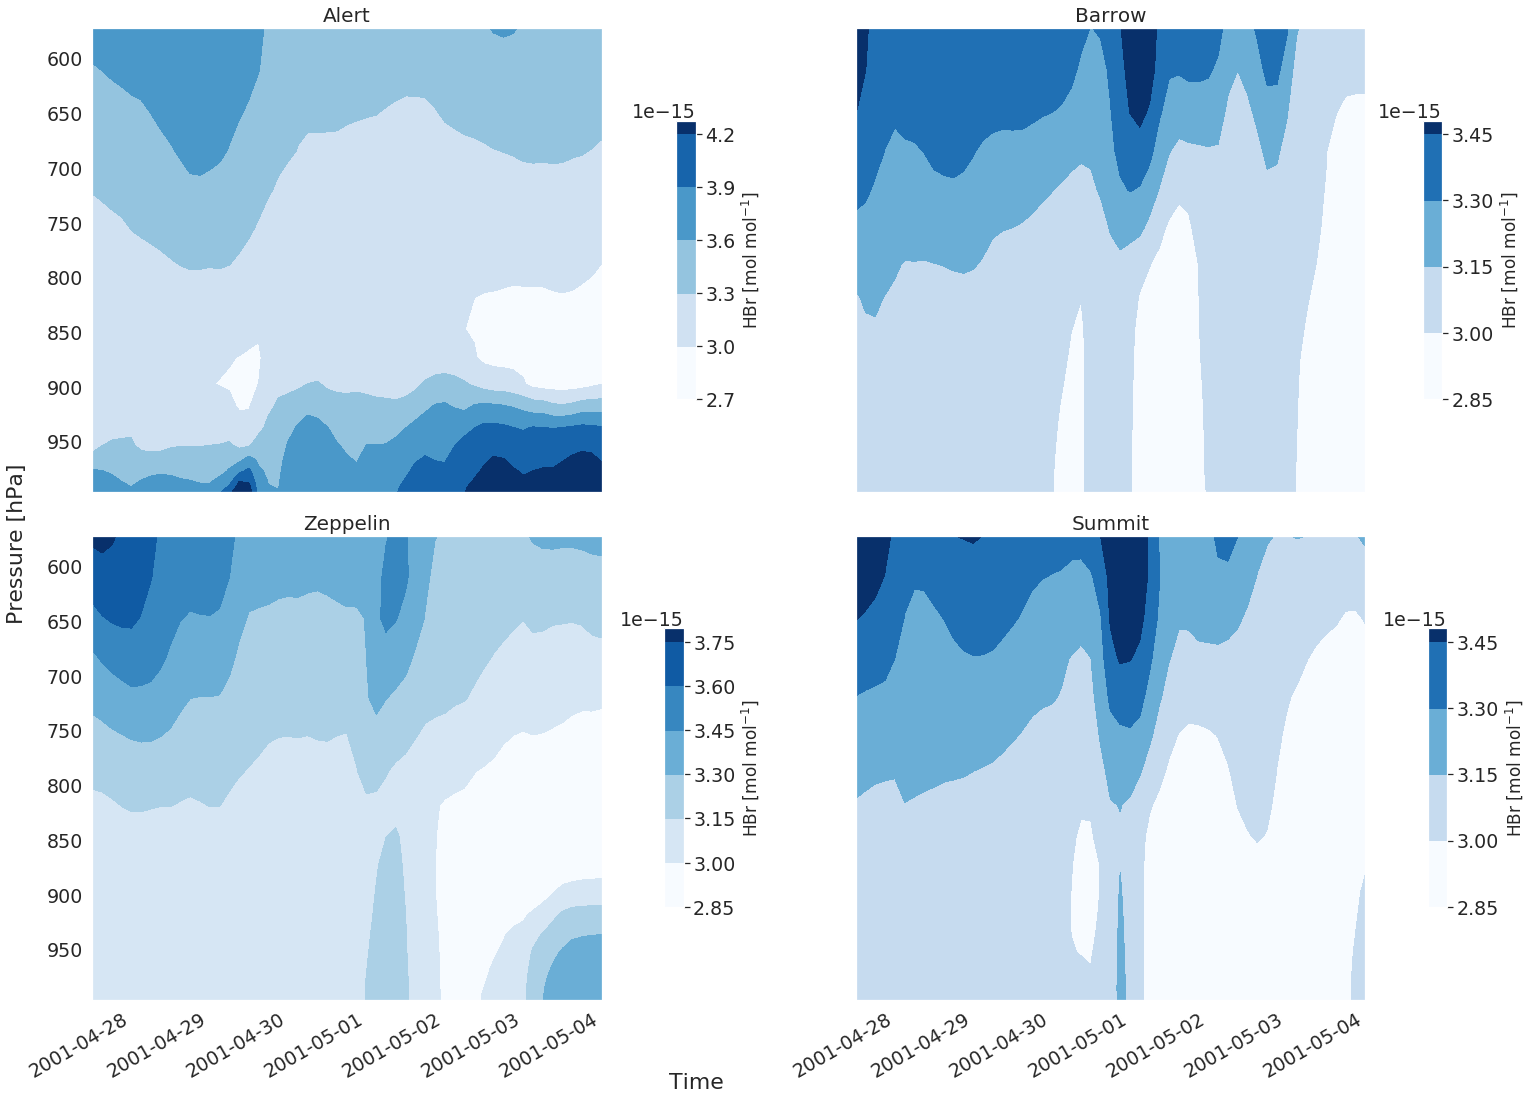
\includegraphics[width = \linewidth]{Chapter6_Results/images/Vert_StationComp_2001/vertHBr_noCl.png}
    \caption{Mixing ratio ($mol mol^{-1}$) of \chem{HBr} in the model layers up to $\sim 600 hPa$ at the four different stations Alert (top left), Barrow (top right), Zeppelin (lower left) and Summit (lower right) in April-May, 2001. The result is from Branch \ref{def:BE_PD_noCl}}
    \label{fig:vertHBr_noCl}
\end{figure}

\begin{figure}[h]
    \centering
    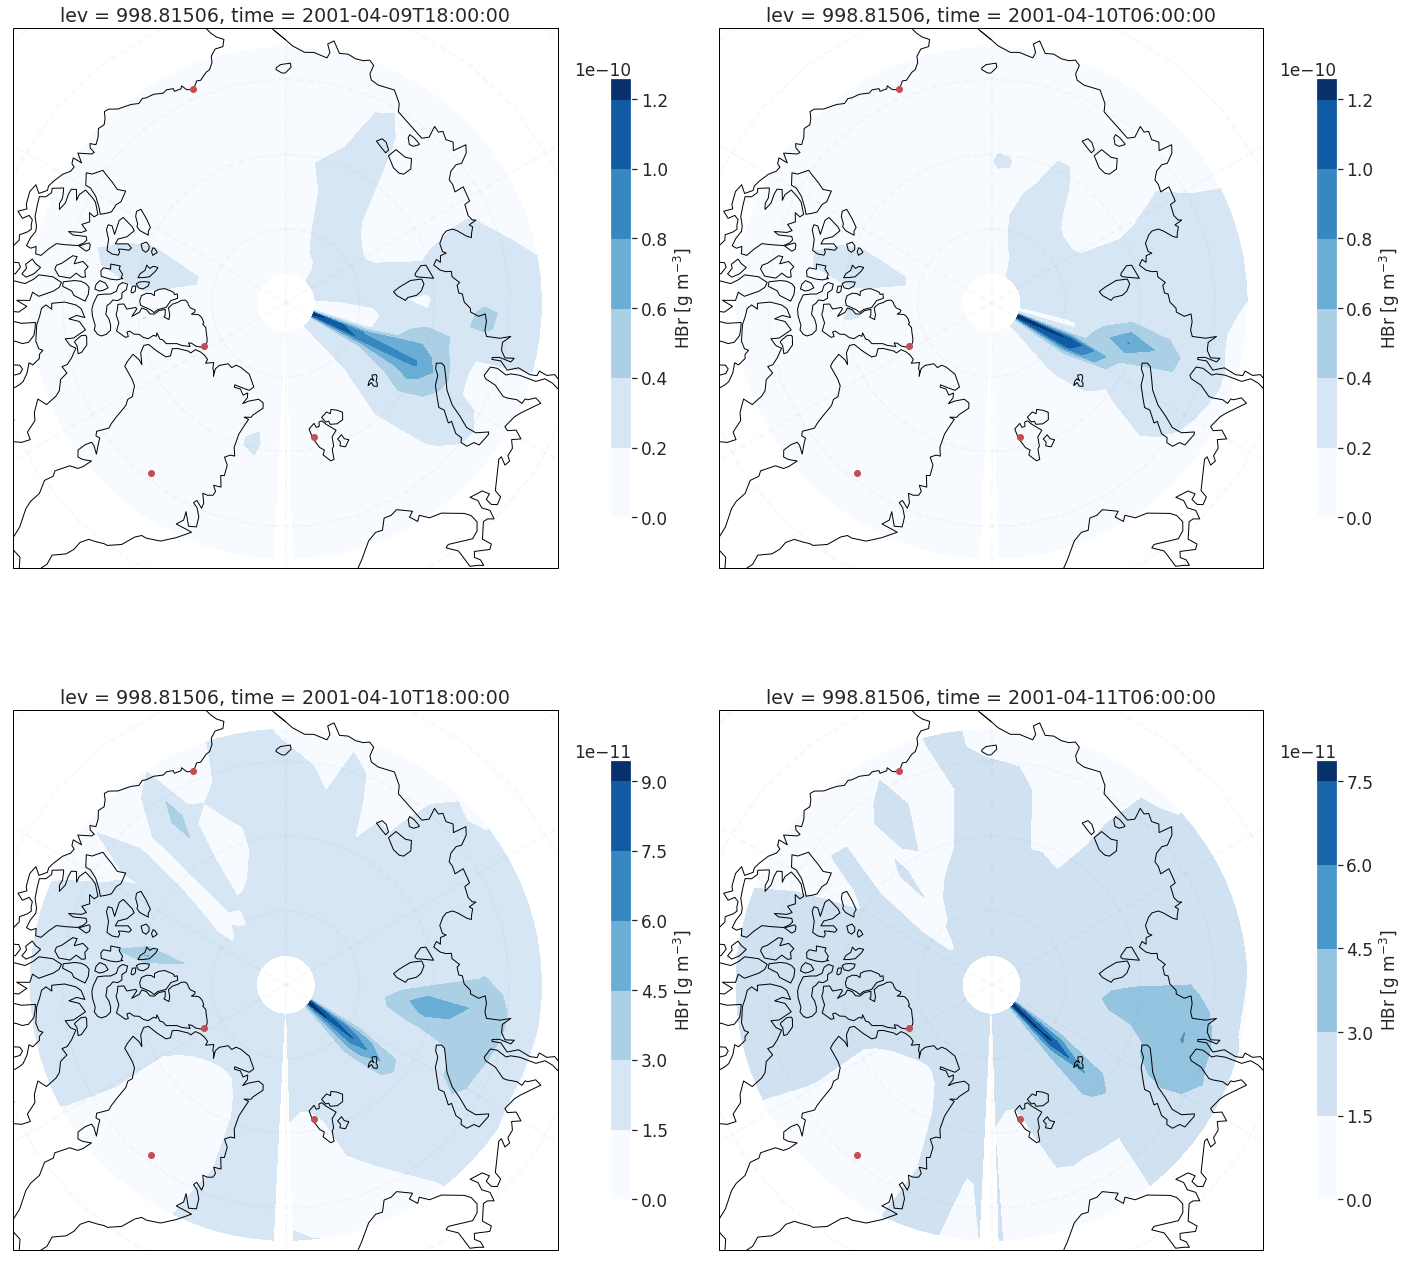
\includegraphics[width = \linewidth]{Chapter6_Results/images/Polar_StationComp_2001/HBr/polarHBr_noCl.png}
    \caption{Concentration ($g m^{-3}$) of \chem{HBr} in the first model layer the Arctic at 18:00 and 06:00 (UTC) of the 9th, 10th and 11th of April, 2001. The result is from Branch \ref{def:BE_PD_noCl} The red dots are the positions of the stations with observations in 2001 (see the map in Figure \ref{fig:stns} for reference)}
    \label{fig:polarHBr_noCl}
\end{figure}

\begin{figure}[h]
    \centering
    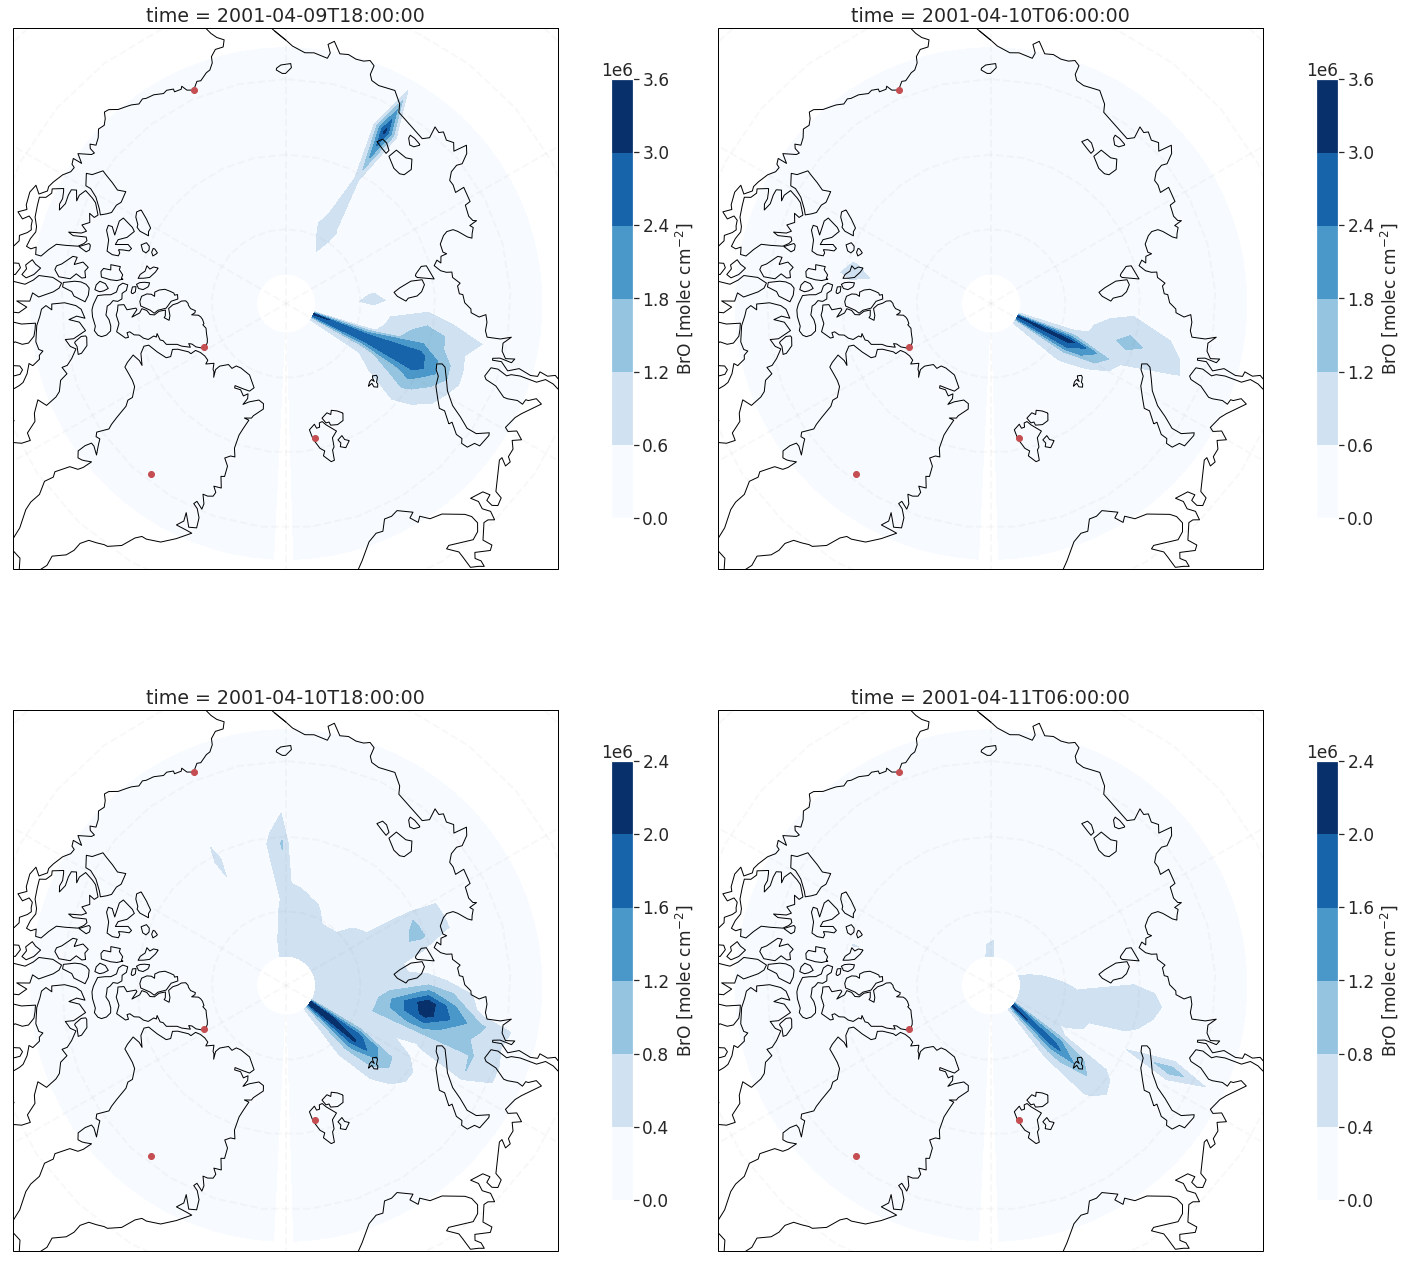
\includegraphics[width = \linewidth]{Chapter6_Results/images/Polar_StationComp_2001/BrO/polarBrO_noCl.png}
    \caption{Vertical column density ($molecules cm^{-2}$) of \chem{BrO} in the lowermost $\sim 250 m$ at 18:00 and 06:00 (UTC) on the 9th, 10th and 11th of April, 2001. The result is from Branch \ref{def:BE_PD_noCl}. The red dots are the positions of the stations with observations in 2001 (see the map in Figure \ref{fig:stns} for reference)}
    \label{fig:polarBrO_noCl}
\end{figure}

\begin{figure}[h]
    \centering
    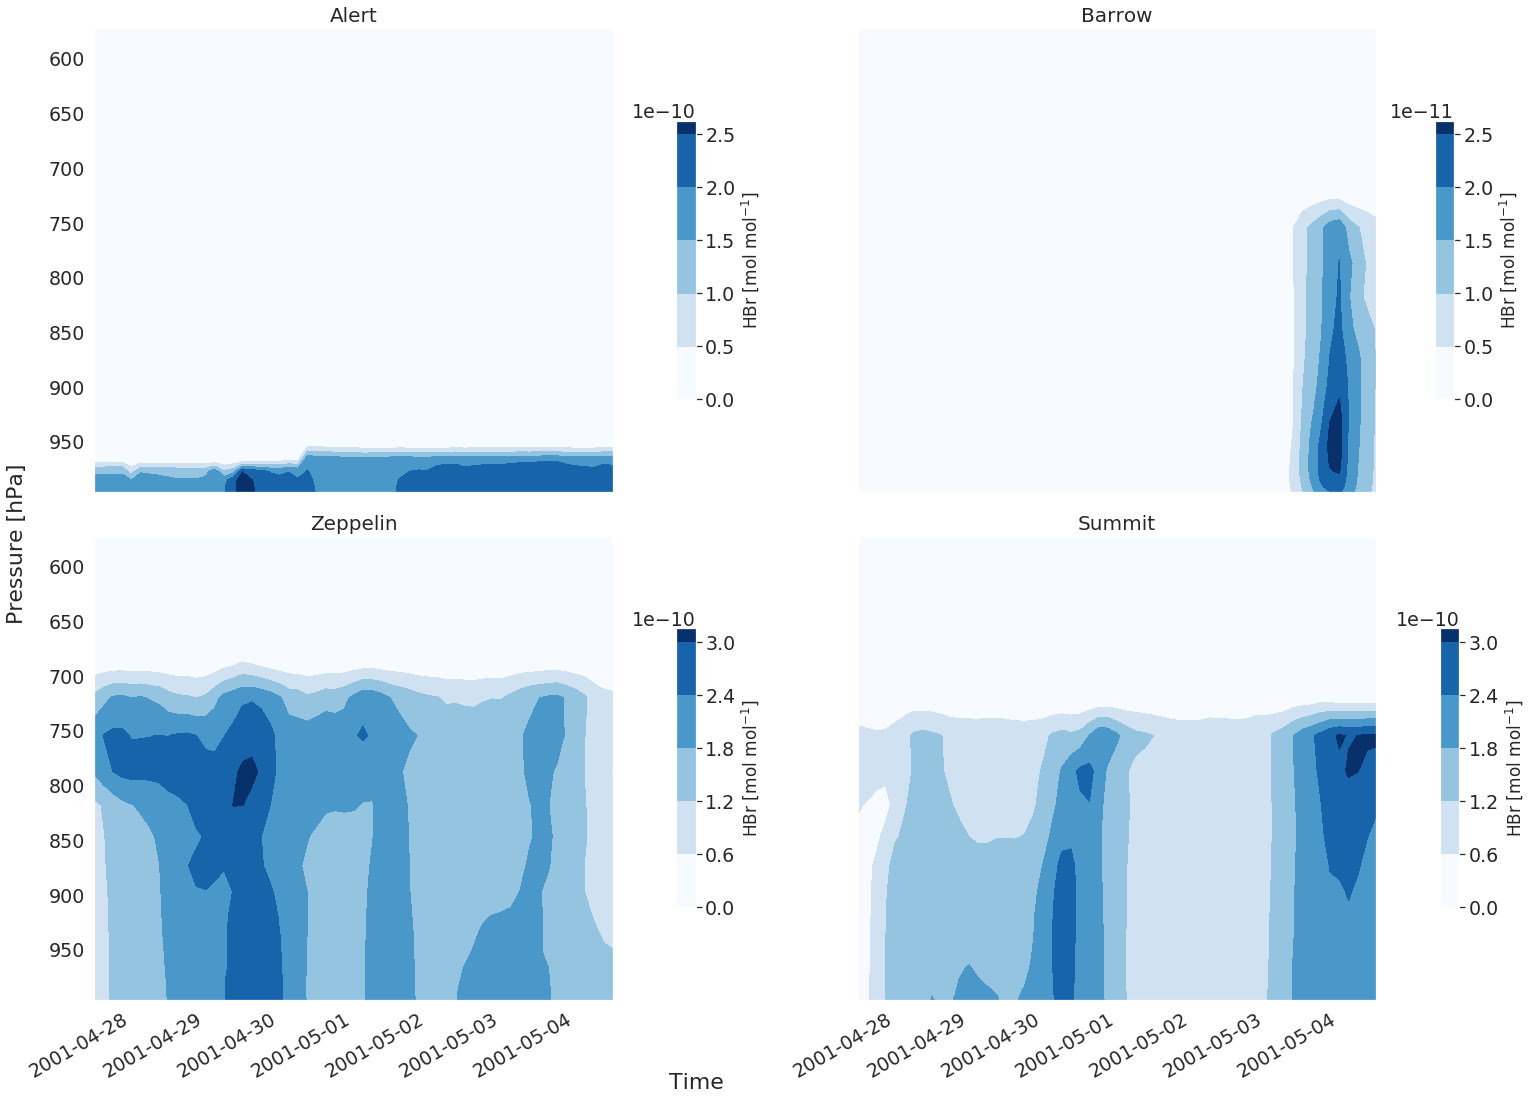
\includegraphics[width=\linewidth]{Chapter6_Results/images/Vert_StationComp_2001/vertHBr_newRestart.png}
    \caption{Mixing ratio ($mol mol^{-1}$) of \chem{HBr} in the model layers up to $\sim 600 hPa$ at the four different stations Alert (top left), Barrow (top right), Zeppelin (lower left) and Summit (lower right) in April-May, 2001. The result is from Branch \ref{def:BE_PD_noCl} initialized with a new restart file with a \chem{HBr} concentration of 10 ppt}
    \label{fig:vertHBr_newRestart}
\end{figure}

\begin{figure}[h]
    \centering
    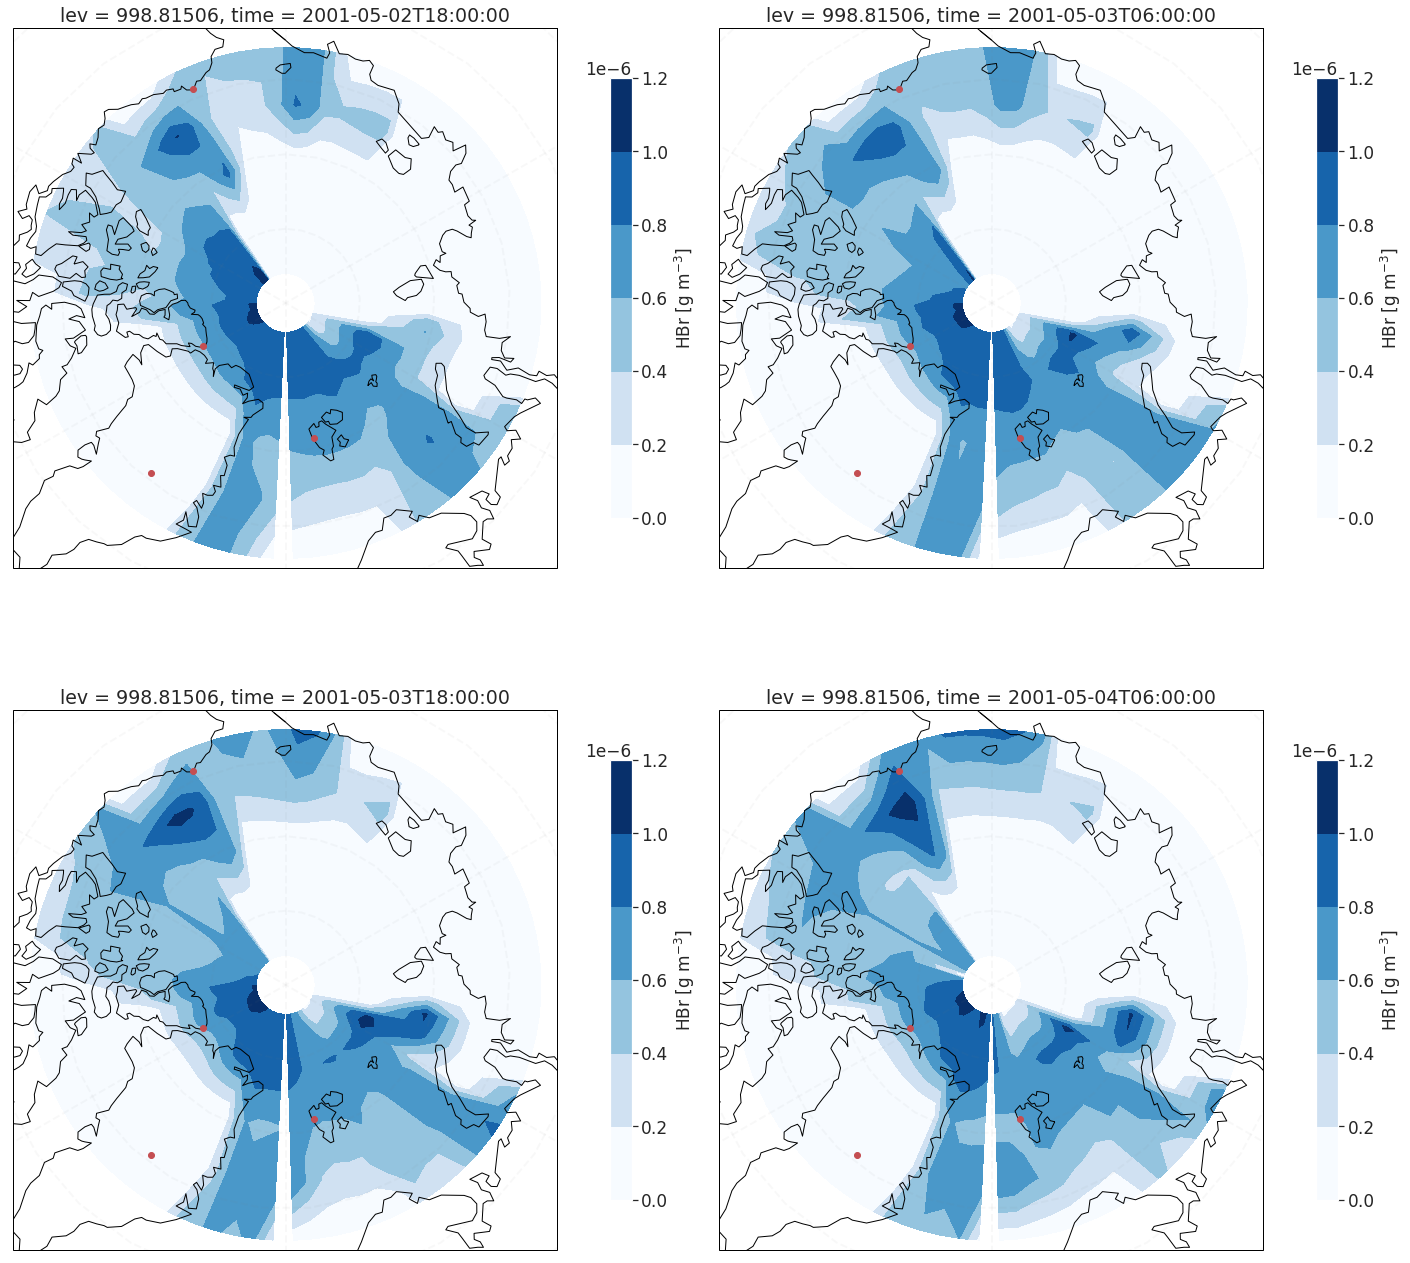
\includegraphics[width=\linewidth]{Chapter6_Results/images/Polar_StationComp_2001/HBr/polarHBr_newRestart.png}
    \caption{Concentration ($g m^{-3}$) of \chem{HBr} in the first model layer the Arctic at 18:00 and 06:00 (UTC) of the 2nd, 3rd and 4th of May, 2001. The result is from Branch \ref{def:BE_PD_noCl} initialized with a new restart file with a \chem{HBr} concentration of 10 ppt. The red dots are the positions of the stations with observations in 2001 (see the map in Figure \ref{fig:stns} for reference)}
    \label{fig:polarHBr_newRestart}
\end{figure}

\begin{figure}[h]
    \centering
    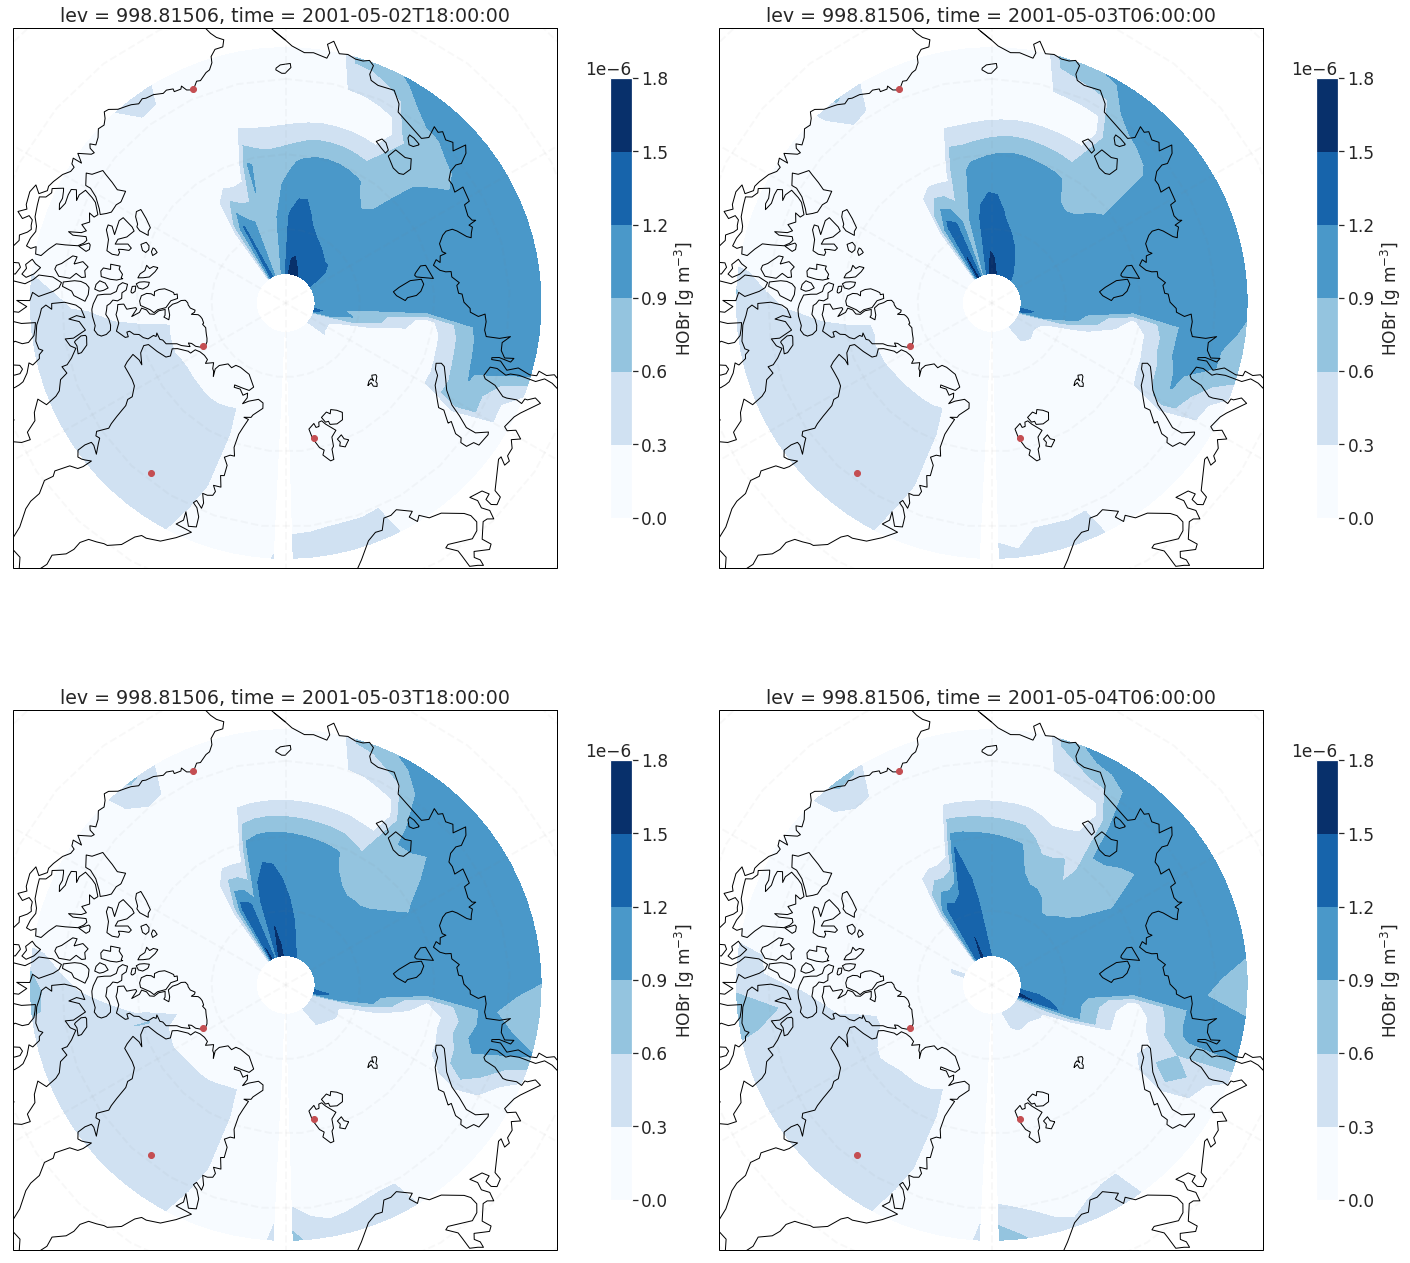
\includegraphics[width=\linewidth]{Chapter6_Results/images/Polar_StationComp_2001/HOBr/polarHOBr_newRestart.png}
    \caption{Concentration ($g m^{-3}$) of \chem{HOBr} in the first model layer the Arctic at 18:00 and 06:00 (UTC) of the 2nd, 3rd and 4th of May, 2001. The result is from Branch \ref{def:BE_PD_noCl} initialized with a new restart file with a \chem{HBr} concentration of 10 ppt. The red dots are the positions of the stations with observations in 2001 (see the map in Figure \ref{fig:stns} for reference)}
    \label{fig:polarHOBr_newRestart}
\end{figure}

\begin{figure}[h]
    \centering
    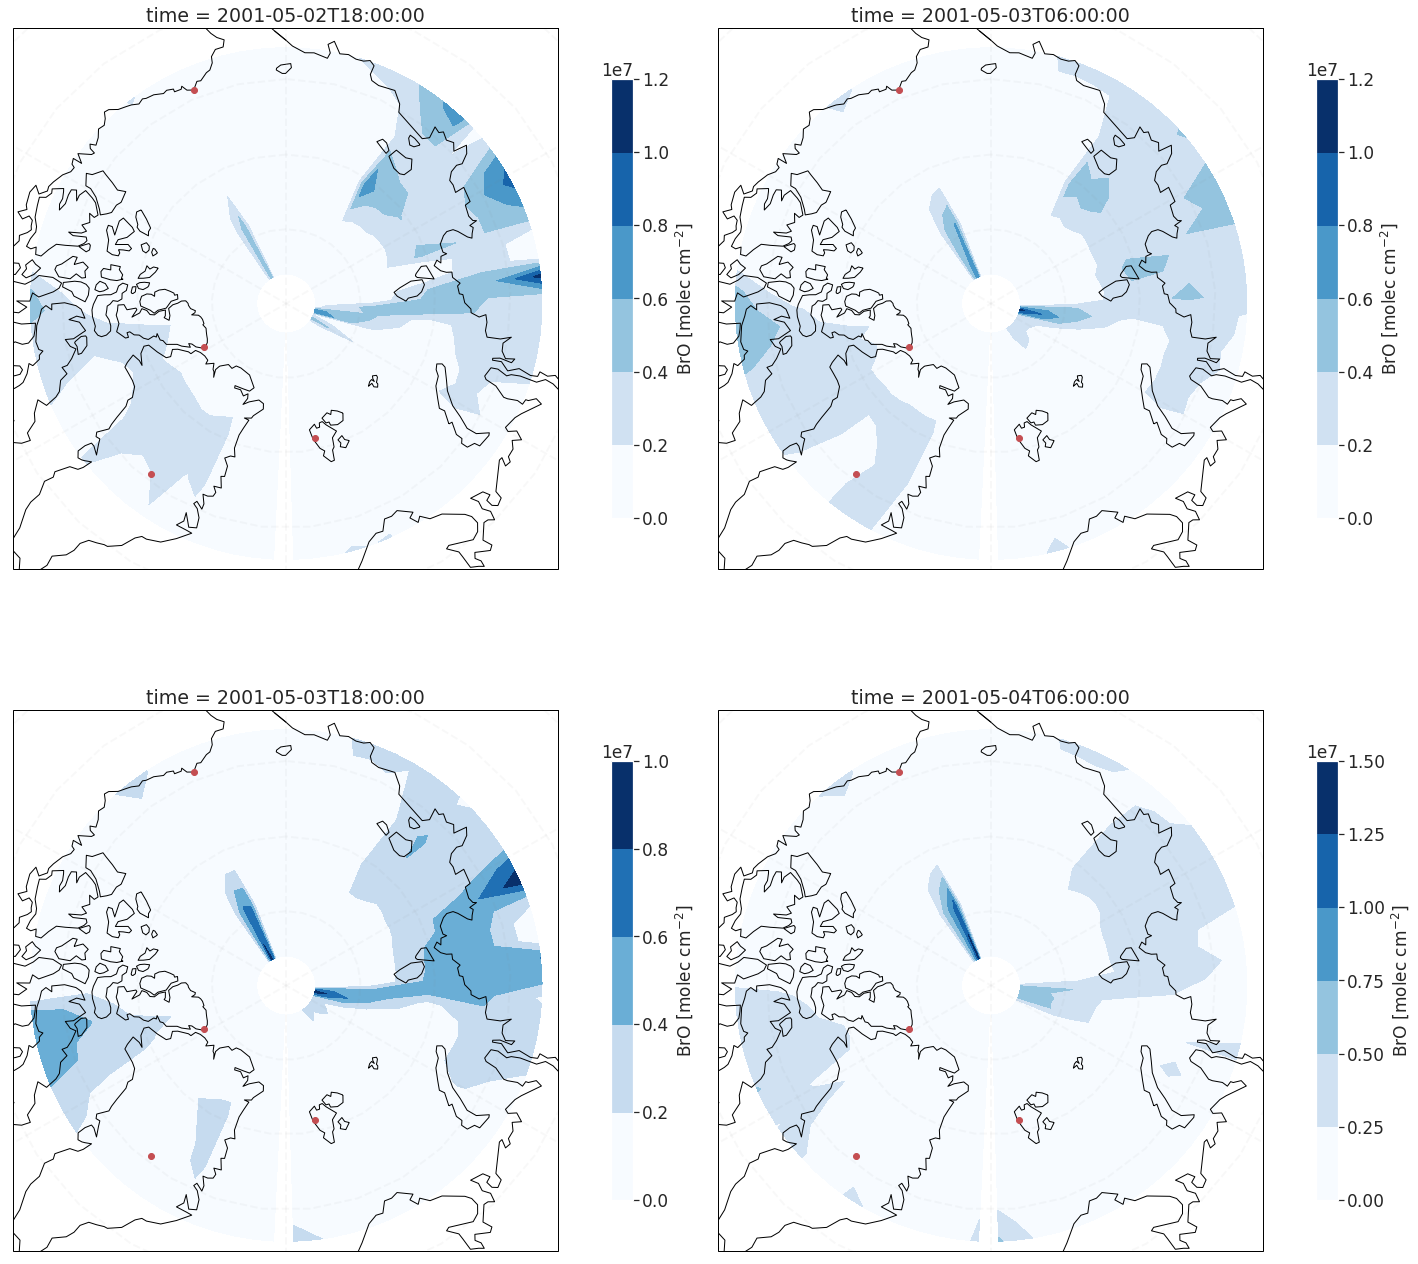
\includegraphics[width=\linewidth]{Chapter6_Results/images/Polar_StationComp_2001/BrO/polarBro_newRestart.png}
    \caption{Vertical column density ($molecules cm^{-2}$) of \chem{BrO} in the lowermost $\sim 250 m$ at 18:00 and 06:00 (UTC) on the  2nd, 3rd and 4th of May, 2001. The result is from Branch \ref{def:BE_PD_noCl} initialized with a new restart file with a \chem{HBr} concentration of 10 ppt. The red dots are the positions of the stations with observations in 2001 (see the map in Figure \ref{fig:stns} for reference)}
    \label{fig:polarBro_newRestart}
\end{figure}

%\begin{figure}[h]
    \centering
    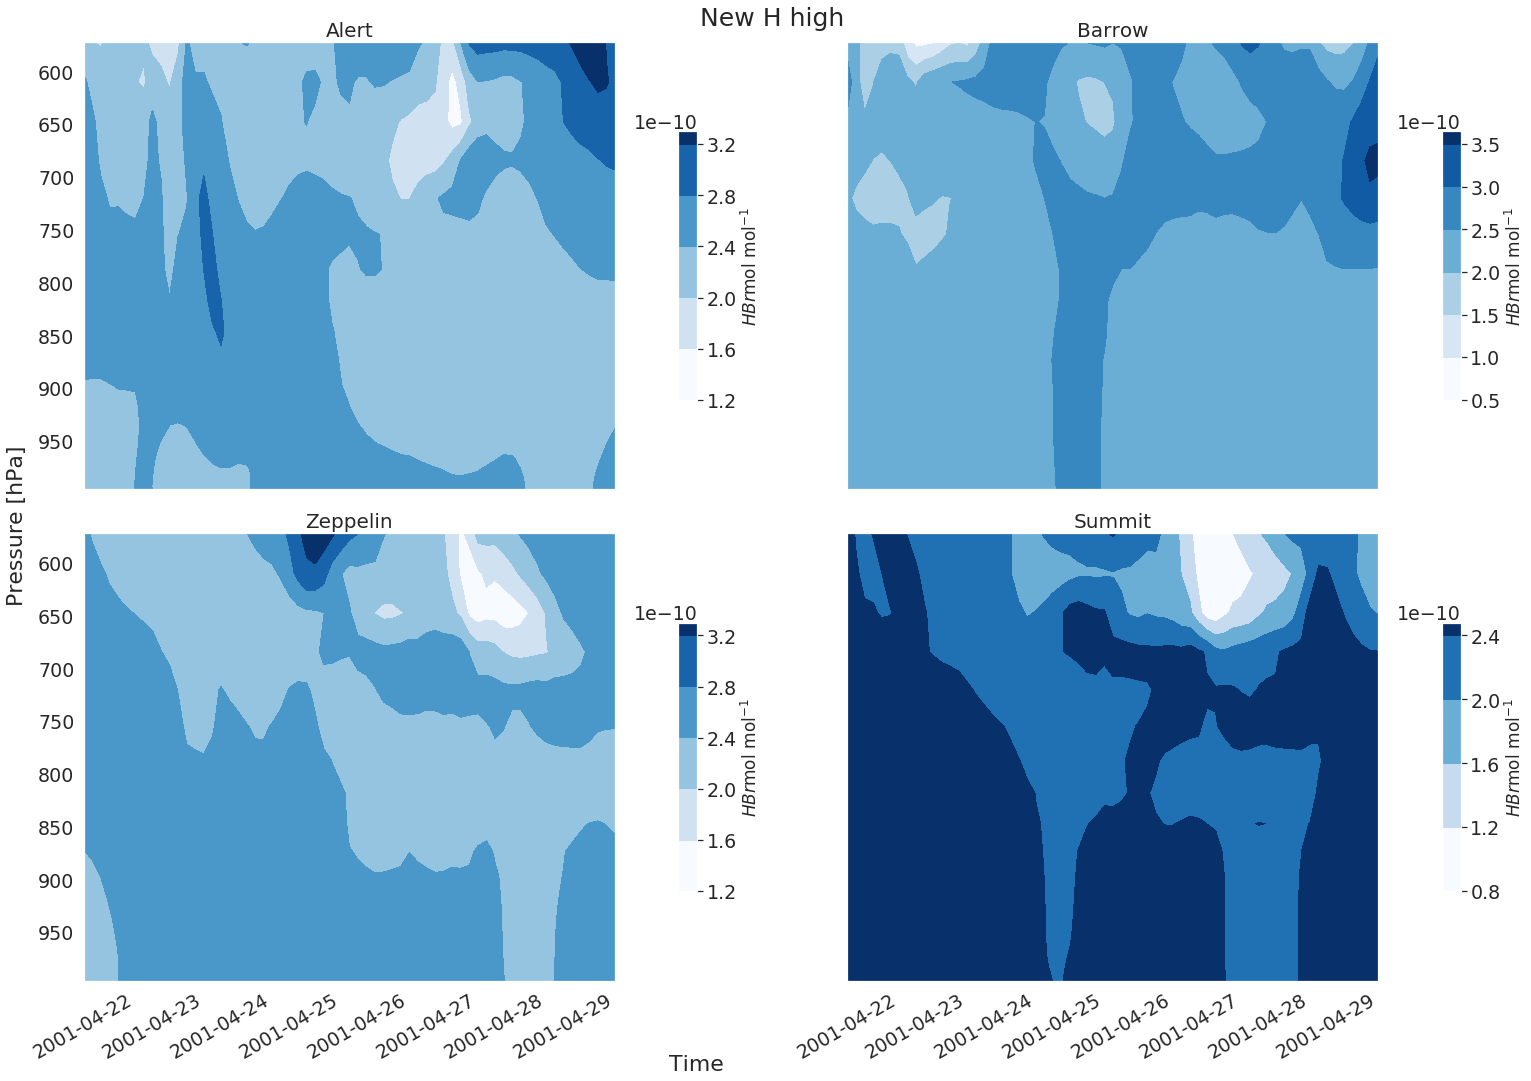
\includegraphics[width=\linewidth]{Chapter6_Results/images/vertHBr_HFOUR_step3.png}
    \caption{Mixing ratio ($mol mol^{-1}$) of \chem{HBr} in the model layers up to $\sim 600 hPa$ at the four different stations Alert (top left), Barrow (top right), Zeppelin (lower left) and Summit (lower right) in April, 2001. The result is from the test including hard-coded photodissociation rates as well as a new (high) Henry-coefficient at HFOUR resolution}
    \label{fig:vertHBr_HFOUR_step3}
\end{figure}
\begin{figure}[h]
    \centering
    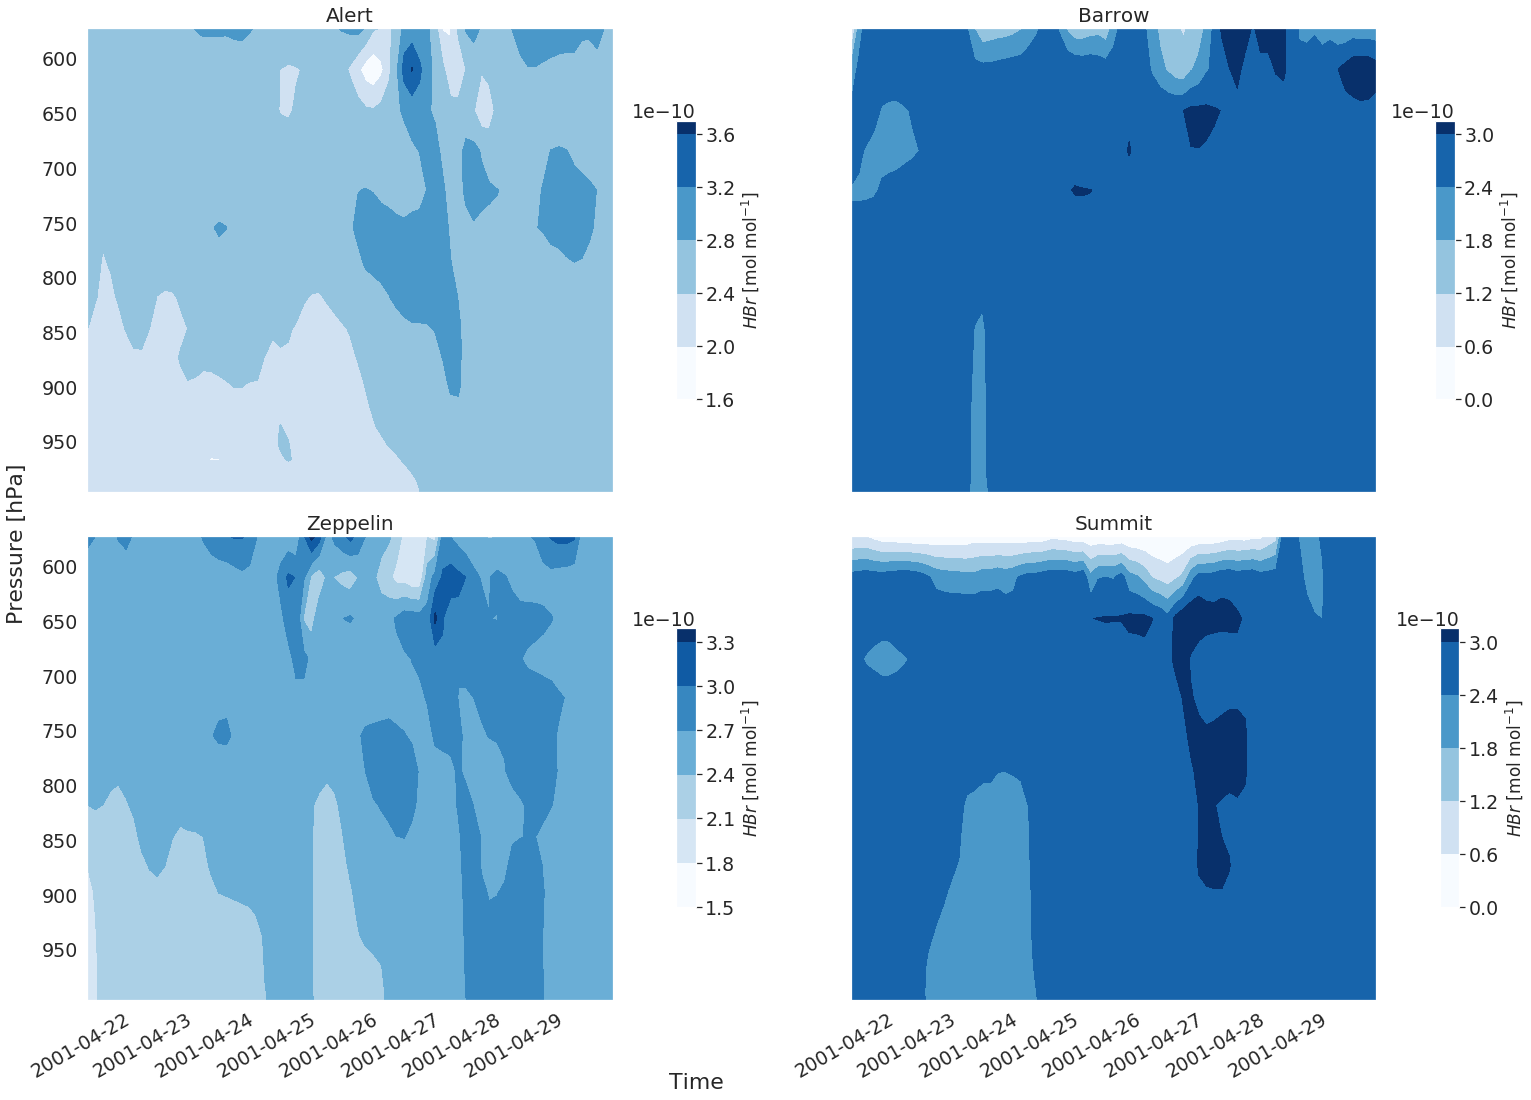
\includegraphics[width=\linewidth]{Chapter6_Results/images/Vert_StationComp_2001/vertHBr_HTWO_step3.png}
    \caption{Mixing ratio ($mol mol^{-1}$) of \chem{HBr} in the model layers up to $\sim 600 hPa$ at the four different stations Alert (top left), Barrow (top right), Zeppelin (lower left) and Summit (lower right) in April, 2001. The result is from Branch \ref{def:BE_PD_noCl} including hard-coded photodissociation rates as well as a new (high) Henry-coefficient at HTWO resolution}
    \label{fig:vertHBr_HTWO_step3}
\end{figure}

%\begin{figure}[h]
    \centering
    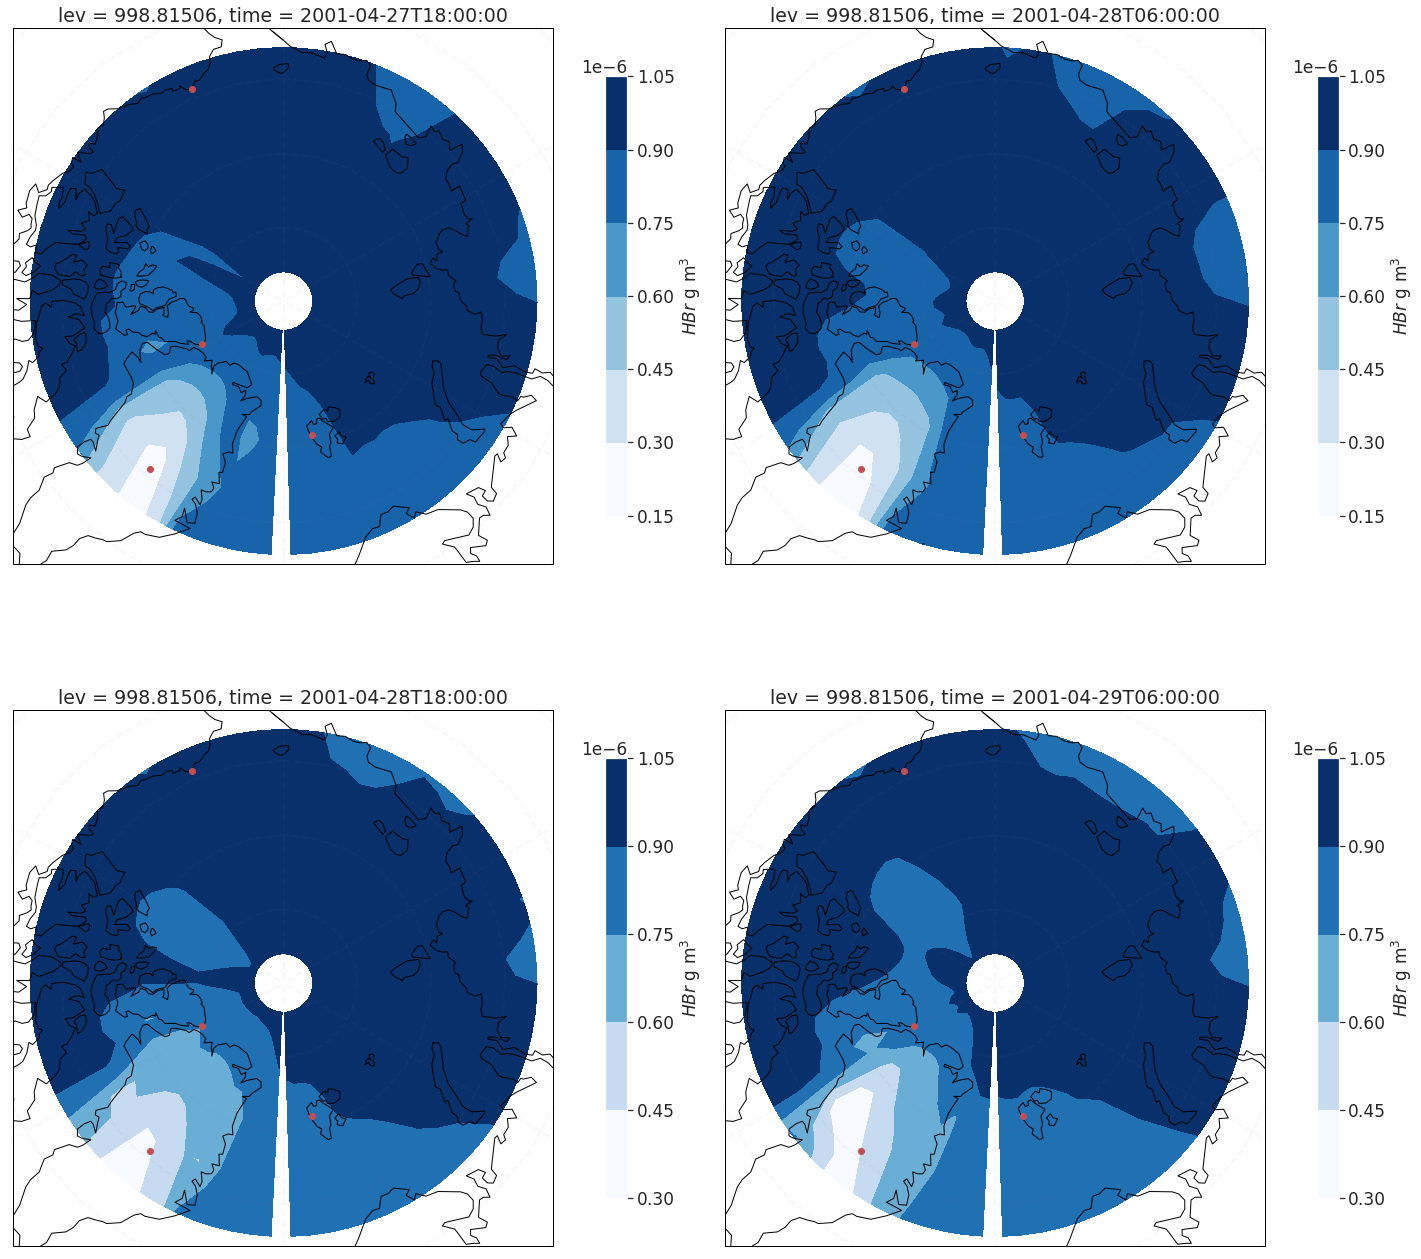
\includegraphics[width=\linewidth]{Chapter6_Results/images/polarHBr_HFOUR_step3.png}
    \caption{Concentration ($g m^{-3}$) of \chem{HBr} in the first model layer the Arctic at 18:00 and 06:00 (UTC) of the 27th, 28th and 29th of April, 2001. The result is from the test including hard-coded photodissociation rates as well as a new (high) Henry-coefficient at HFOUR resolution. The red dots are the positions of the stations with observations in 2001 (see the map in Figure \ref{fig:stns} for reference)}
    \label{fig:polarHBr_HFOUR_step3}
\end{figure}
\begin{figure}[h]
    \centering
    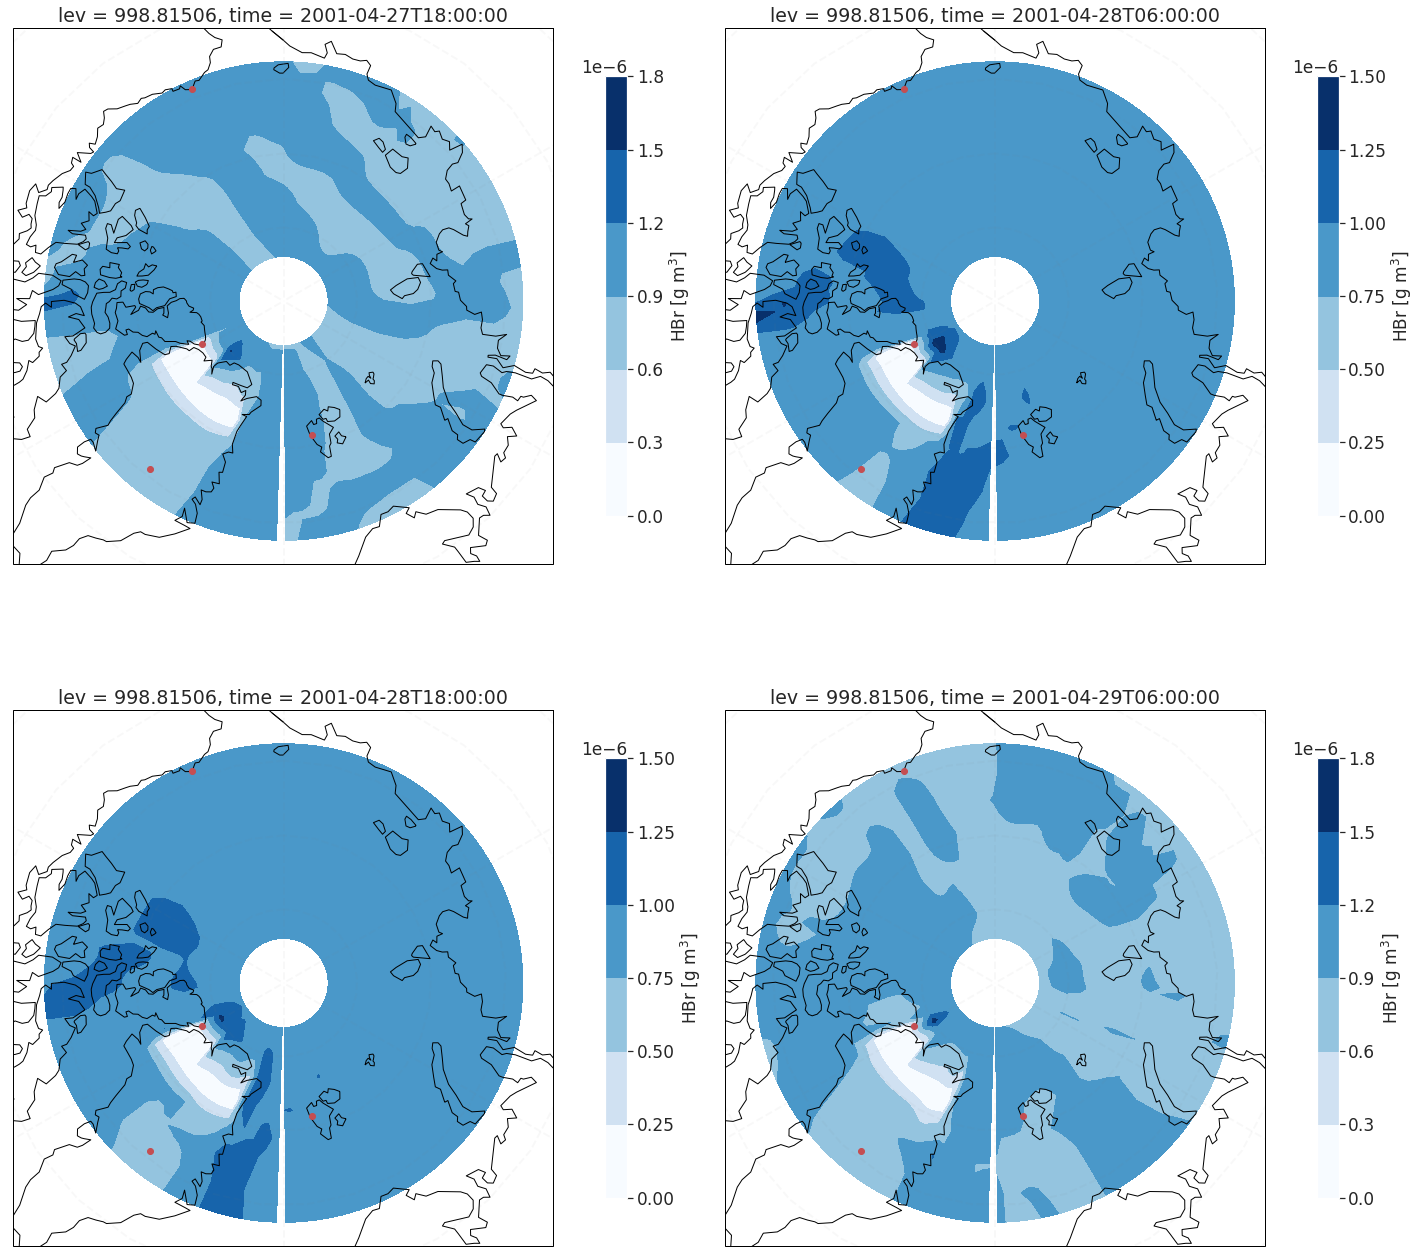
\includegraphics[width=\linewidth]{Chapter6_Results/images/Polar_StationComp_2001/HBr/polarHBr_HTWO_step3.png}
    \caption{Concentration ($g m^{-3}$) of \chem{HBr} in the first model layer the Arctic at 18:00 and 06:00 (UTC) of the 27th, 28th and 29th of April, 2001. The result is from Branch \ref{def:BE_PD_noCl} including hard-coded photodissociation rates as well as a new (high) Henry-coefficient at HTWO resolution. The red dots are the positions of the stations with observations in 2001 (see the map in Figure \ref{fig:stns} for reference)}
    \label{fig:polarHBr_HTWO_step3}
\end{figure}

\begin{figure}[h]
    \centering
    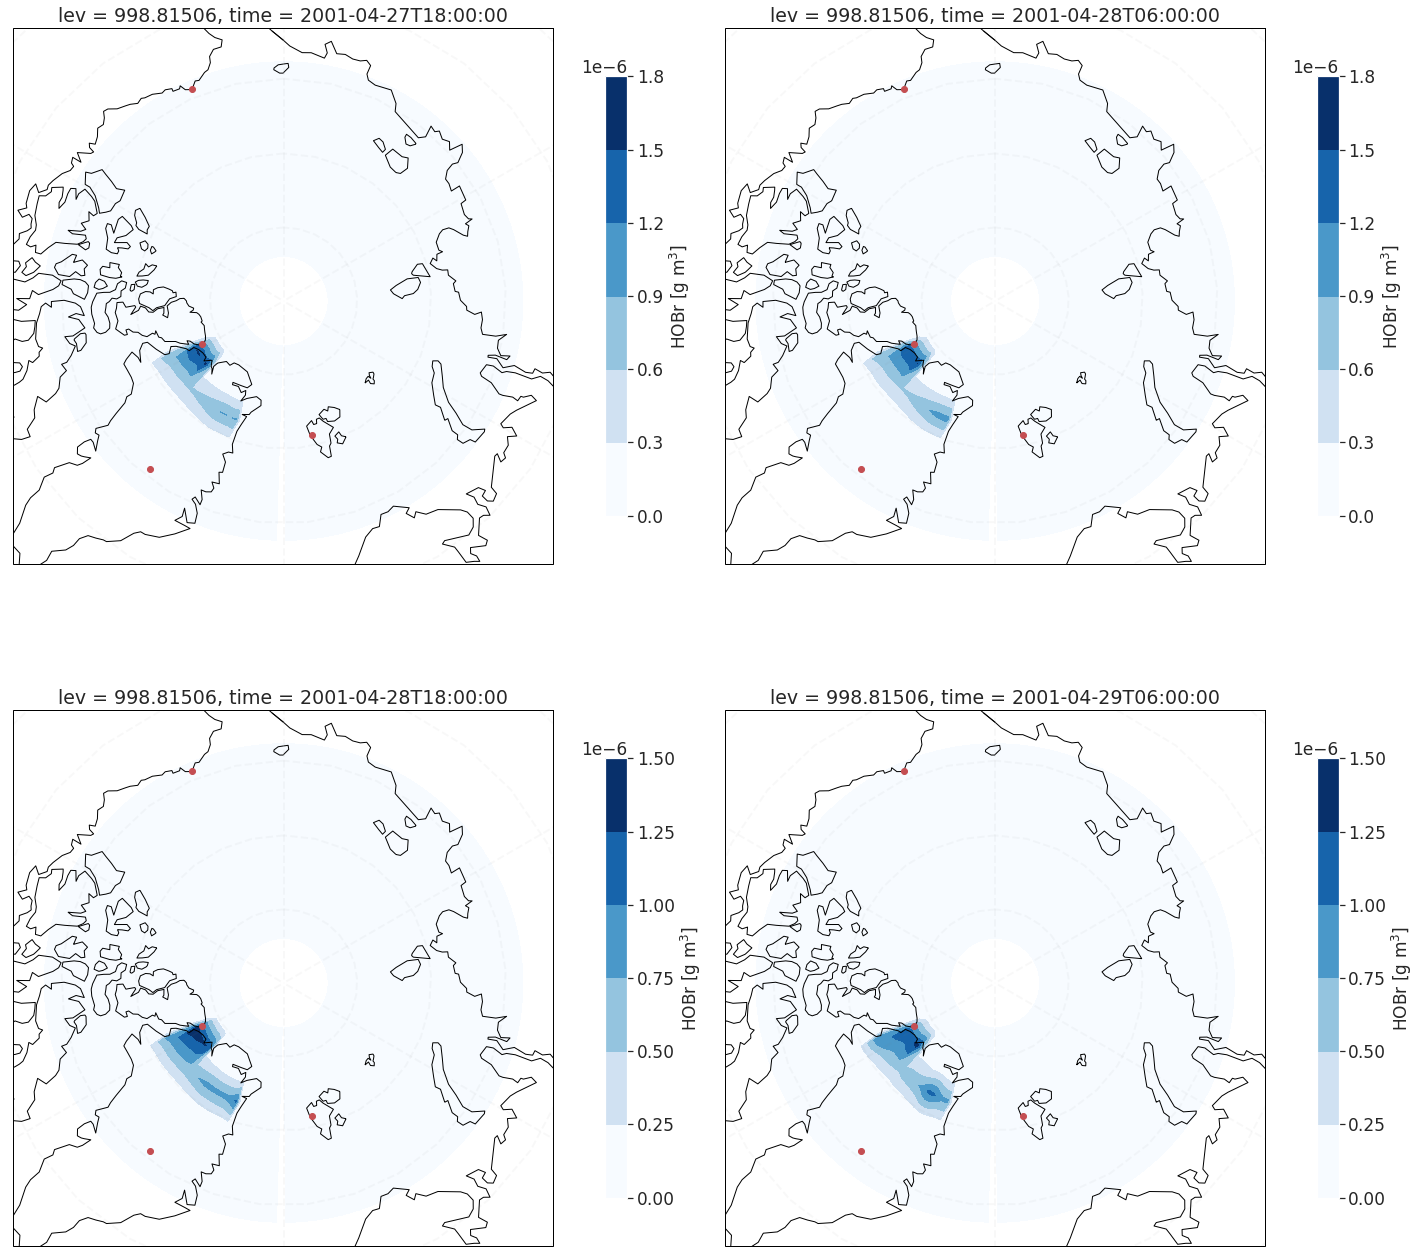
\includegraphics[width=\linewidth]{Chapter6_Results/images/Polar_StationComp_2001/HOBr/polarHOBr_HTWO_step3.png}
    \caption{Concentration ($g m^{-3}$) of \chem{HOBr} in the first model layer the Arctic at 18:00 and 06:00 (UTC) of the 27th, 28th and 29th of April, 2001. The result is from  Branch \ref{def:BE_PD_noCl} including hard-coded photodissociation rates as well as a new (high) Henry-coefficient at HTWO resolution. The red dots are the positions of the stations with observations in 2001 (see the map in Figure \ref{fig:stns} for reference)}
    \label{fig:polarHOBr_HTWO_step3}
\end{figure}
%\begin{figure}[h]
    \centering
    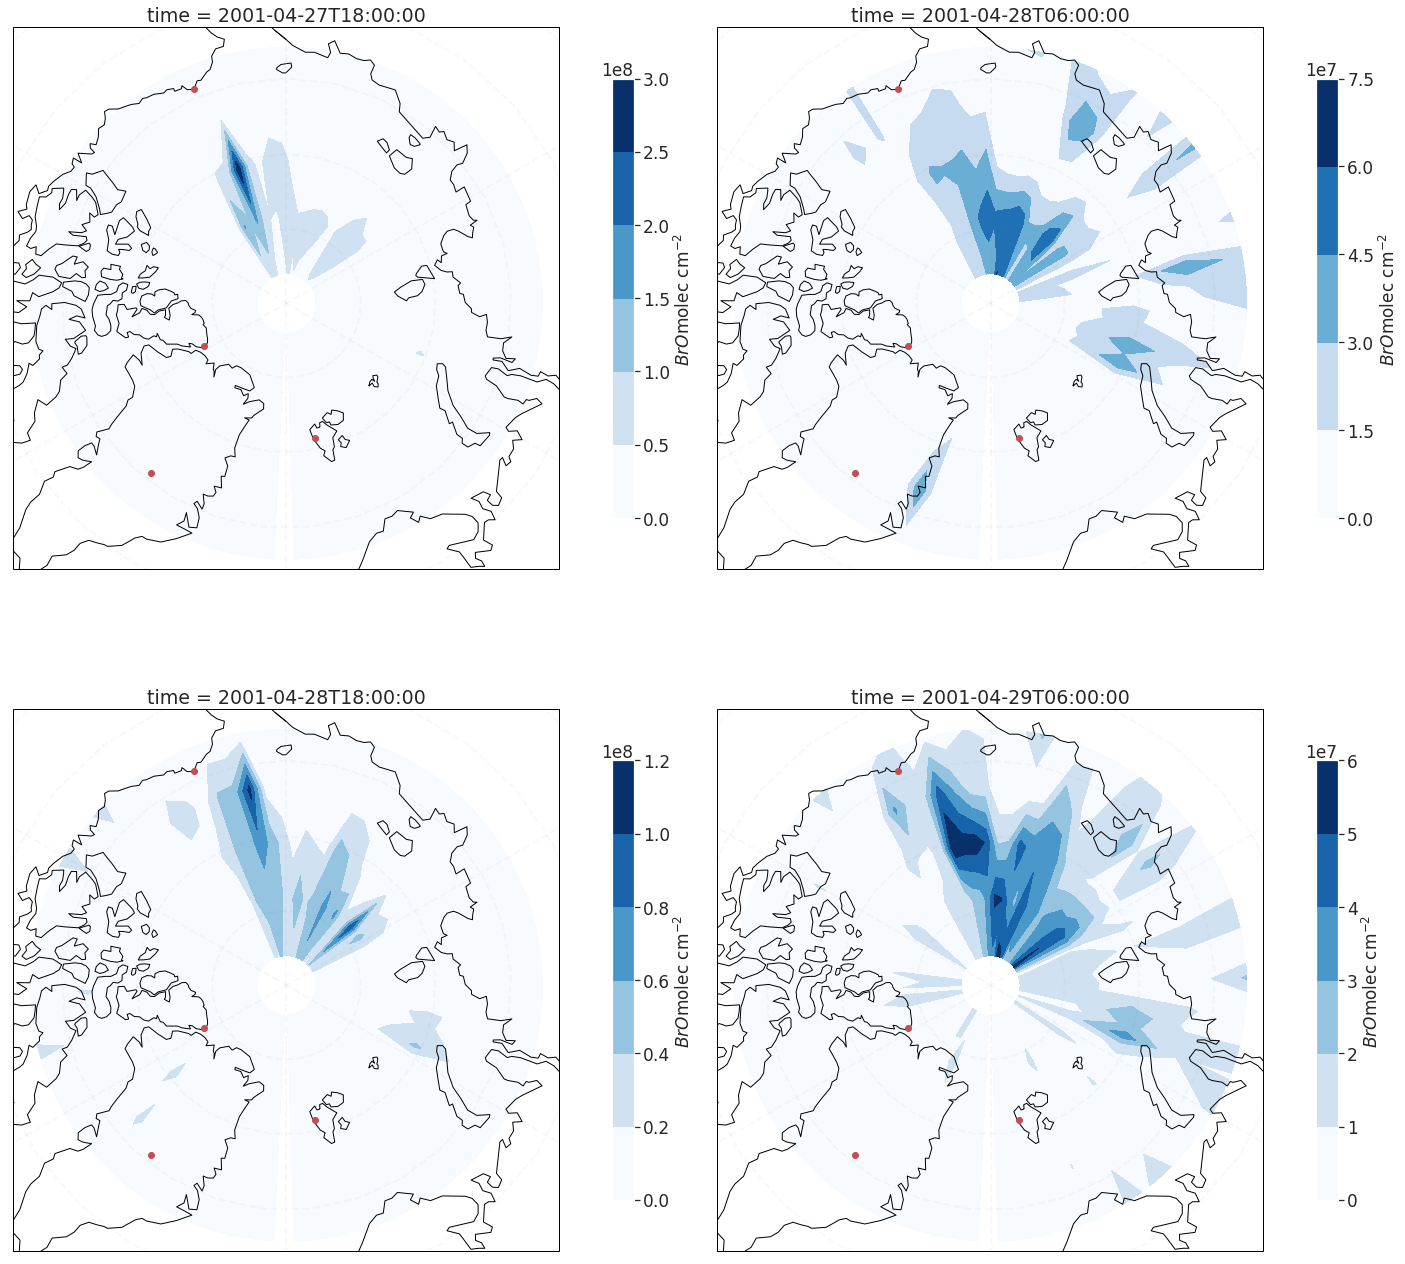
\includegraphics[width=\linewidth]{Chapter6_Results/images/polarBrO_HFOUR_step3.png}
    \caption{Vertical column density ($molecules cm^{-2}$) of \chem{BrO} in the lowermost $\sim 250 m$ at 18:00 and 06:00 (UTC) of the 27th, 28th and 29th of April, 2001. The result is from the test including hard-coded photodissociation rates as well as a new (high) Henry-coefficient at HFOUR resolution. The red dots are the positions of the stations with observations in 2001 (see the map in Figure \ref{fig:stns} for reference)}
    \label{fig:polarBrO_HFOUR_step3}
\end{figure}
\begin{figure}[h]
    \centering
    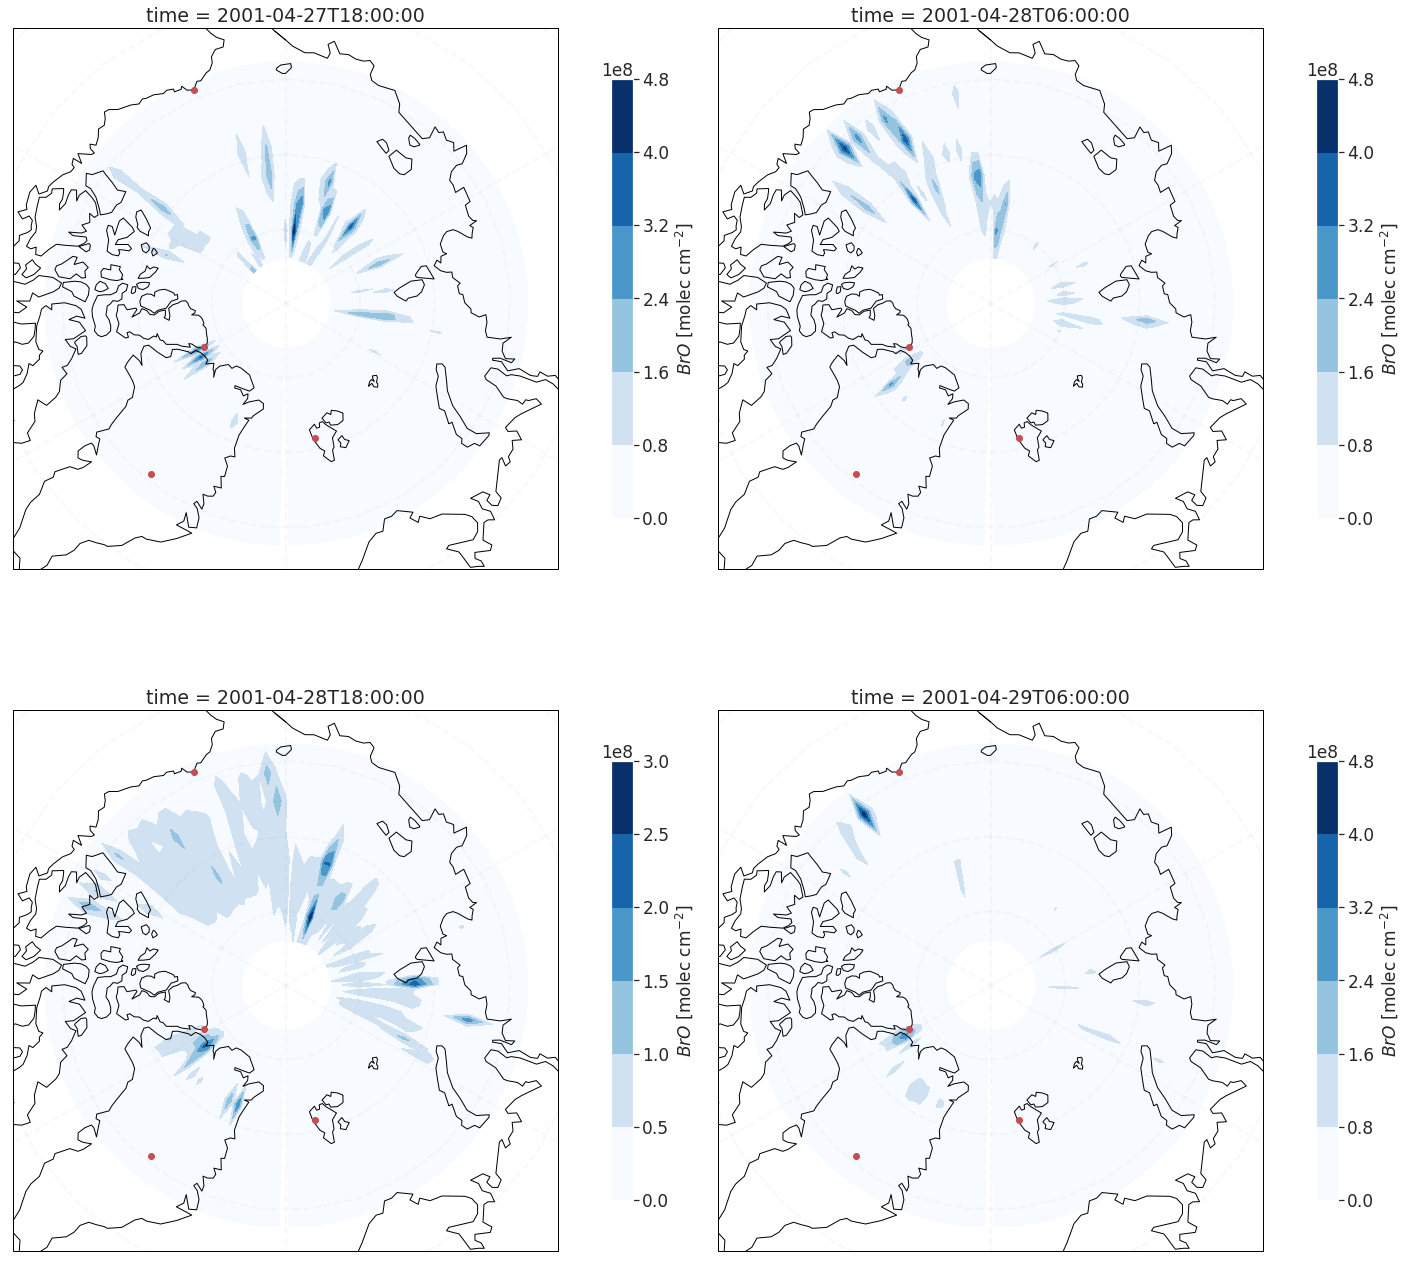
\includegraphics[width=\linewidth]{Chapter6_Results/images/Polar_StationComp_2001/BrO/polarBrO_HTWO_step3.png}
    \caption{Vertical column density ($molecules cm^{-2}$) of \chem{BrO} in the lowermost $\sim 250 m$ at 18:00 and 06:00 (UTC) of the 27th, 28th and 29th of April, 2001. The result is from  Branch \ref{def:BE_PD_noCl} including hard-coded photodissociation rates as well as a new (high) Henry-coefficient at HFOUR resolution. The red dots are the positions of the stations with observations in 2001 (see the map in Figure \ref{fig:stns} for reference)}
    \label{fig:polarBrO_HTWO_step3}
\end{figure}

\clearpage
\section{Analysis of the Final Version of the Halogen Branch}\label{app:final_version}

\begin{figure}[h]
    \centering
    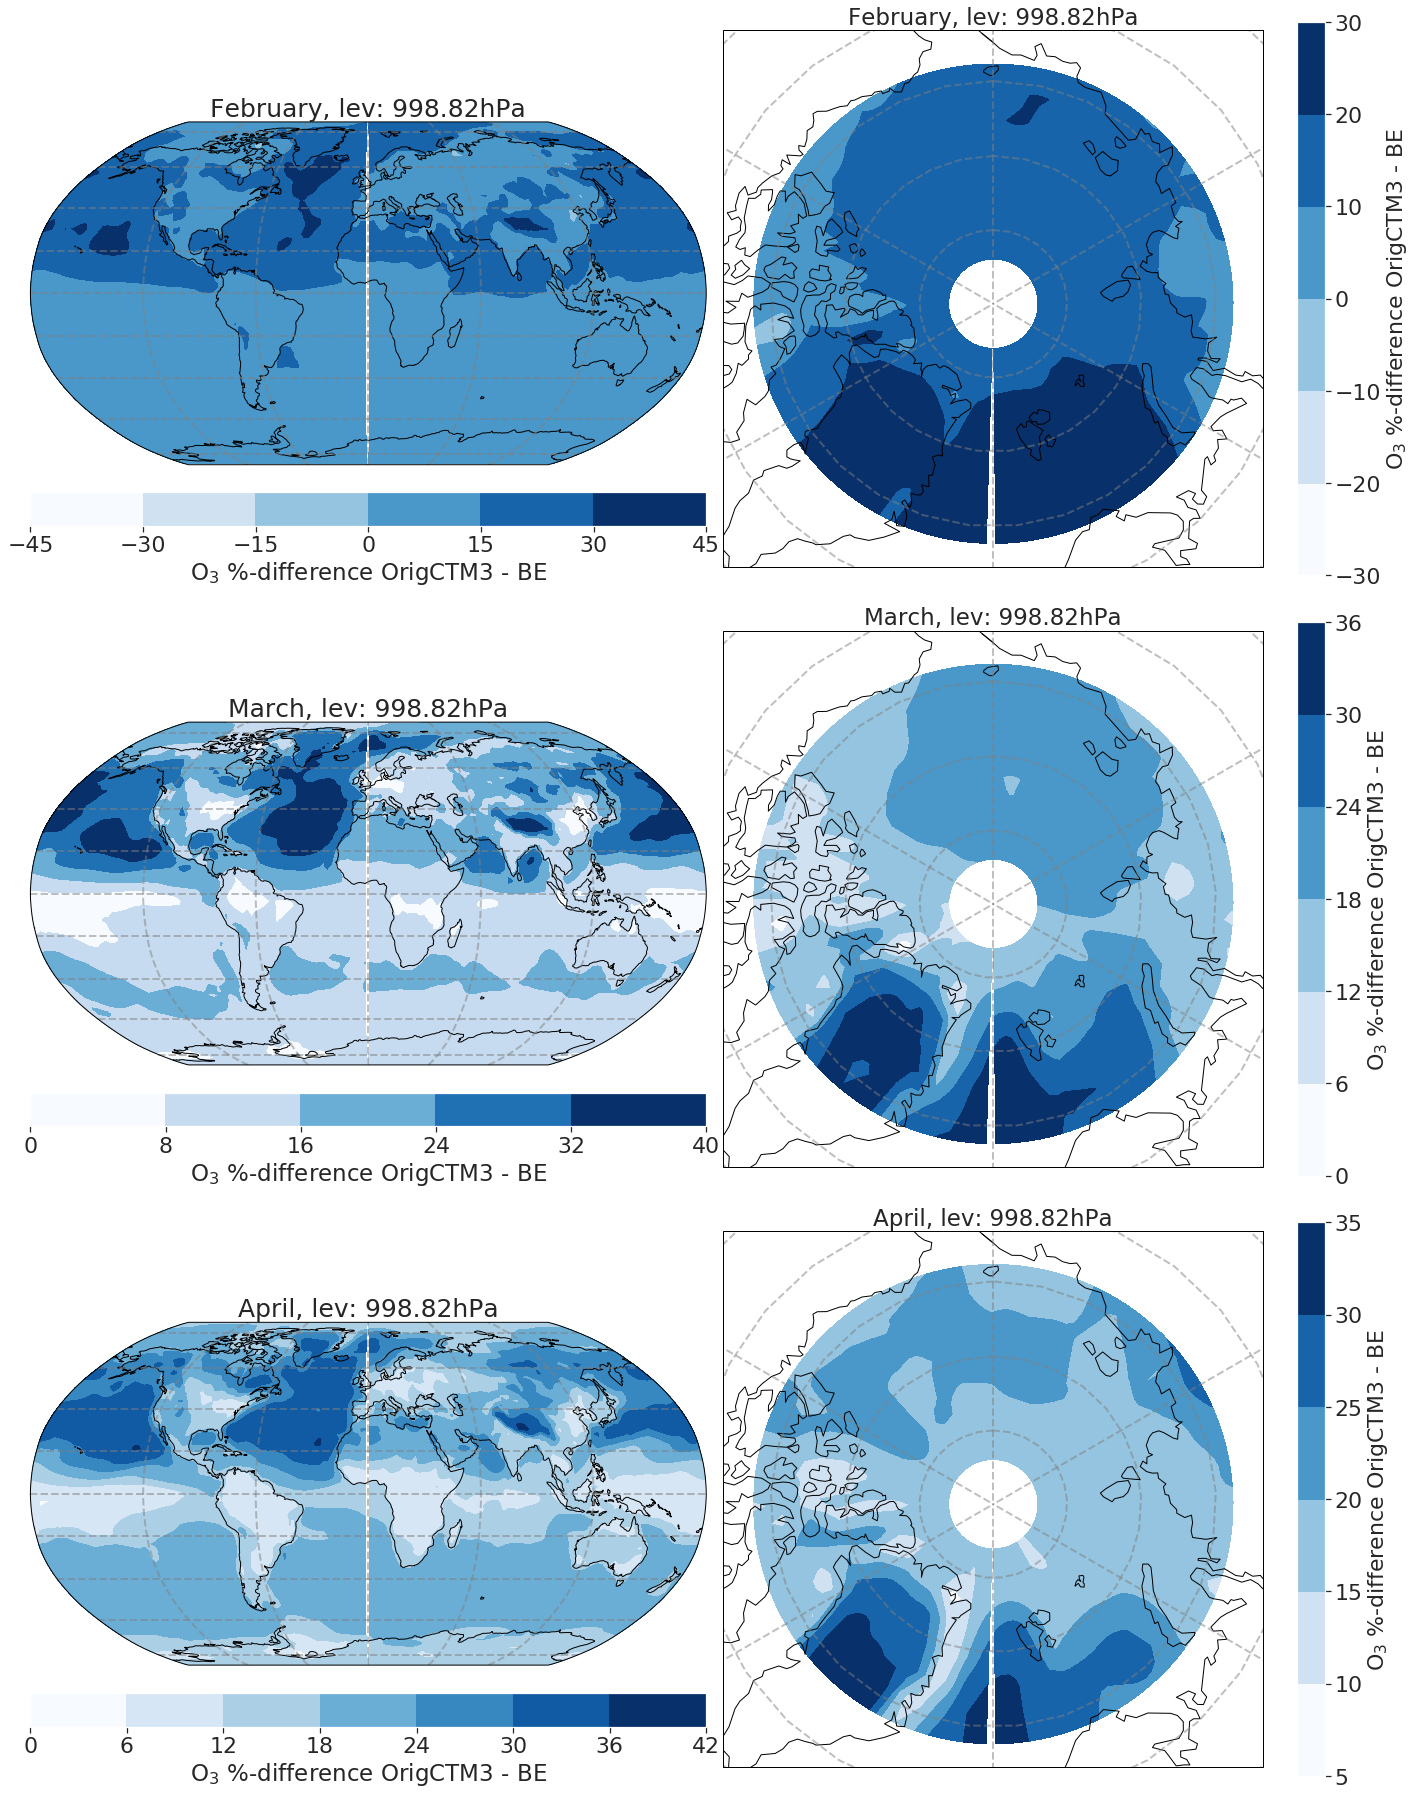
\includegraphics[width = \linewidth]{Chapter6_Results/images/Orig_BE_comp/BE_origPD_vmr_lev0_FebApr_2001.png}
    \caption{Difference in ozone monthly mean volume mixing ratio (in ppb) in the first model layer between the original CTM3 and the BE-branch globally (left columns) and in the Arctic (right columns) in the months February (top figures), March (middle figures) and April (bottom figures) in 2001. \textbf{Note:} the colorbar axis are not equal}
    \label{fig:BE_origPD_vmr_FebApr}
\end{figure}


%%% SKAL TIL APPENDIX

\begin{figure}[h]
    \centering
    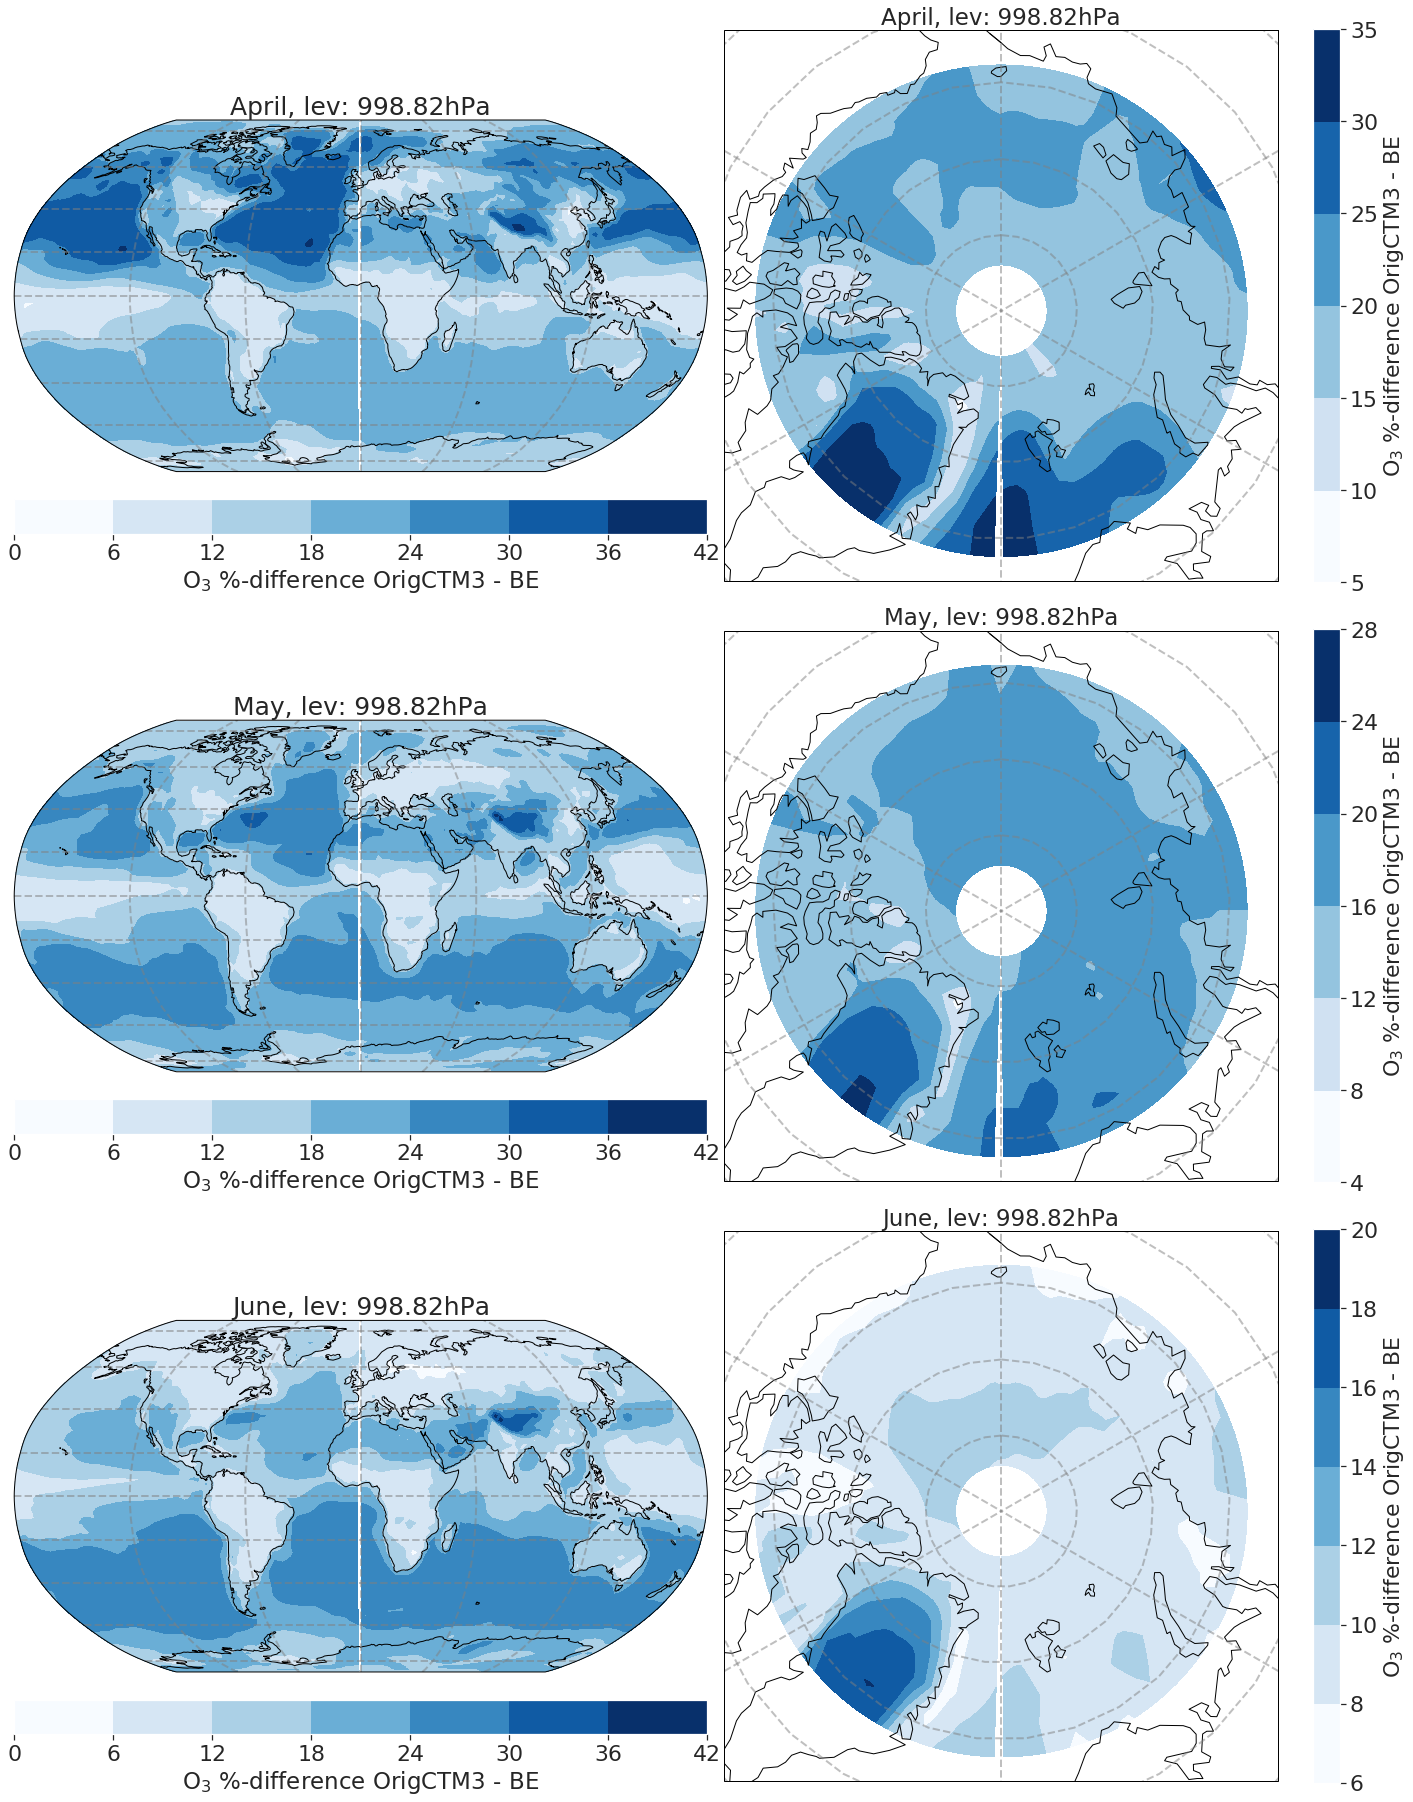
\includegraphics[width = \linewidth]{Chapter6_Results/images/Orig_BE_comp/BE_origPD_vmr_lev0_AprJune_2001.png}
    \caption{Difference in ozone monthly mean volume mixing ratio (in ppb) in the first model layer between the original CTM3 and the BE-branch globally (left columns) and in the Arctic (right columns) in the months April (top figures), May (middle figures) and June (bottom figures) in 2001 \textbf{Note:} the colorbar axis are not equal}
    \label{fig:BE_origPD_vmr_AprJun}
\end{figure}


%%% SKAL TIL APPENDIX

\begin{figure}[h]
    \centering
    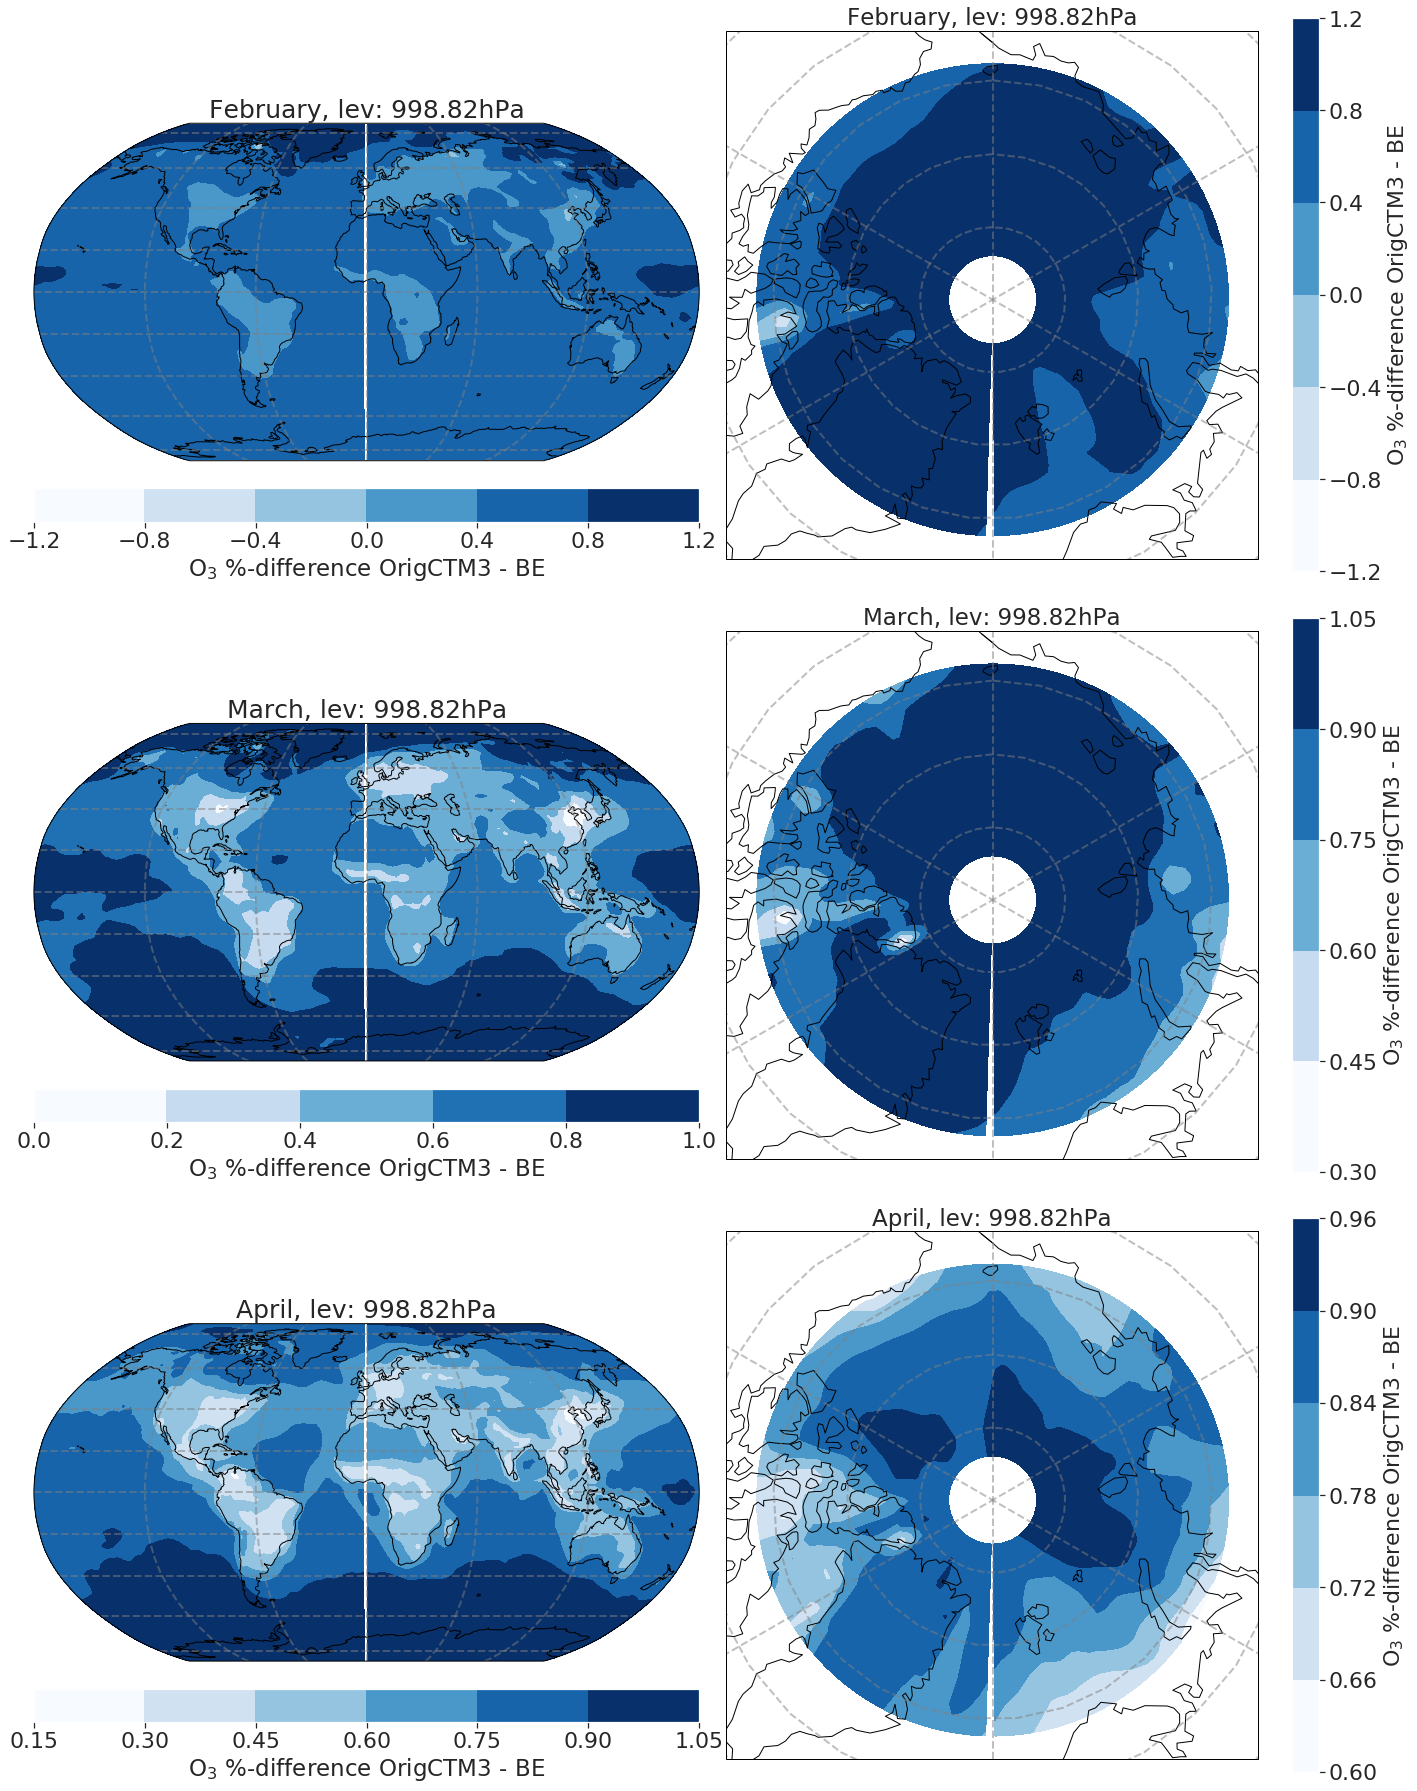
\includegraphics[width = \linewidth]{Chapter6_Results/images/Orig_BE_comp/BE_origPD_percent_lev0_FebApr_2001.png}
    \caption{Percentage difference in ozone monthly mean in the first model layer between the original CTM3 and the BE-branch globally (left columns) and in the Arctic (right columns) in the months February (top figures), March (middle figures) and April (bottom figures) in 2001 \textbf{Note:} the colorbar axis are not equal}
    \label{fig:BE_origPD_percent_FebApr}
\end{figure}


%%% SKAL TIL APPENDIX

\begin{figure}[h]
    \centering
    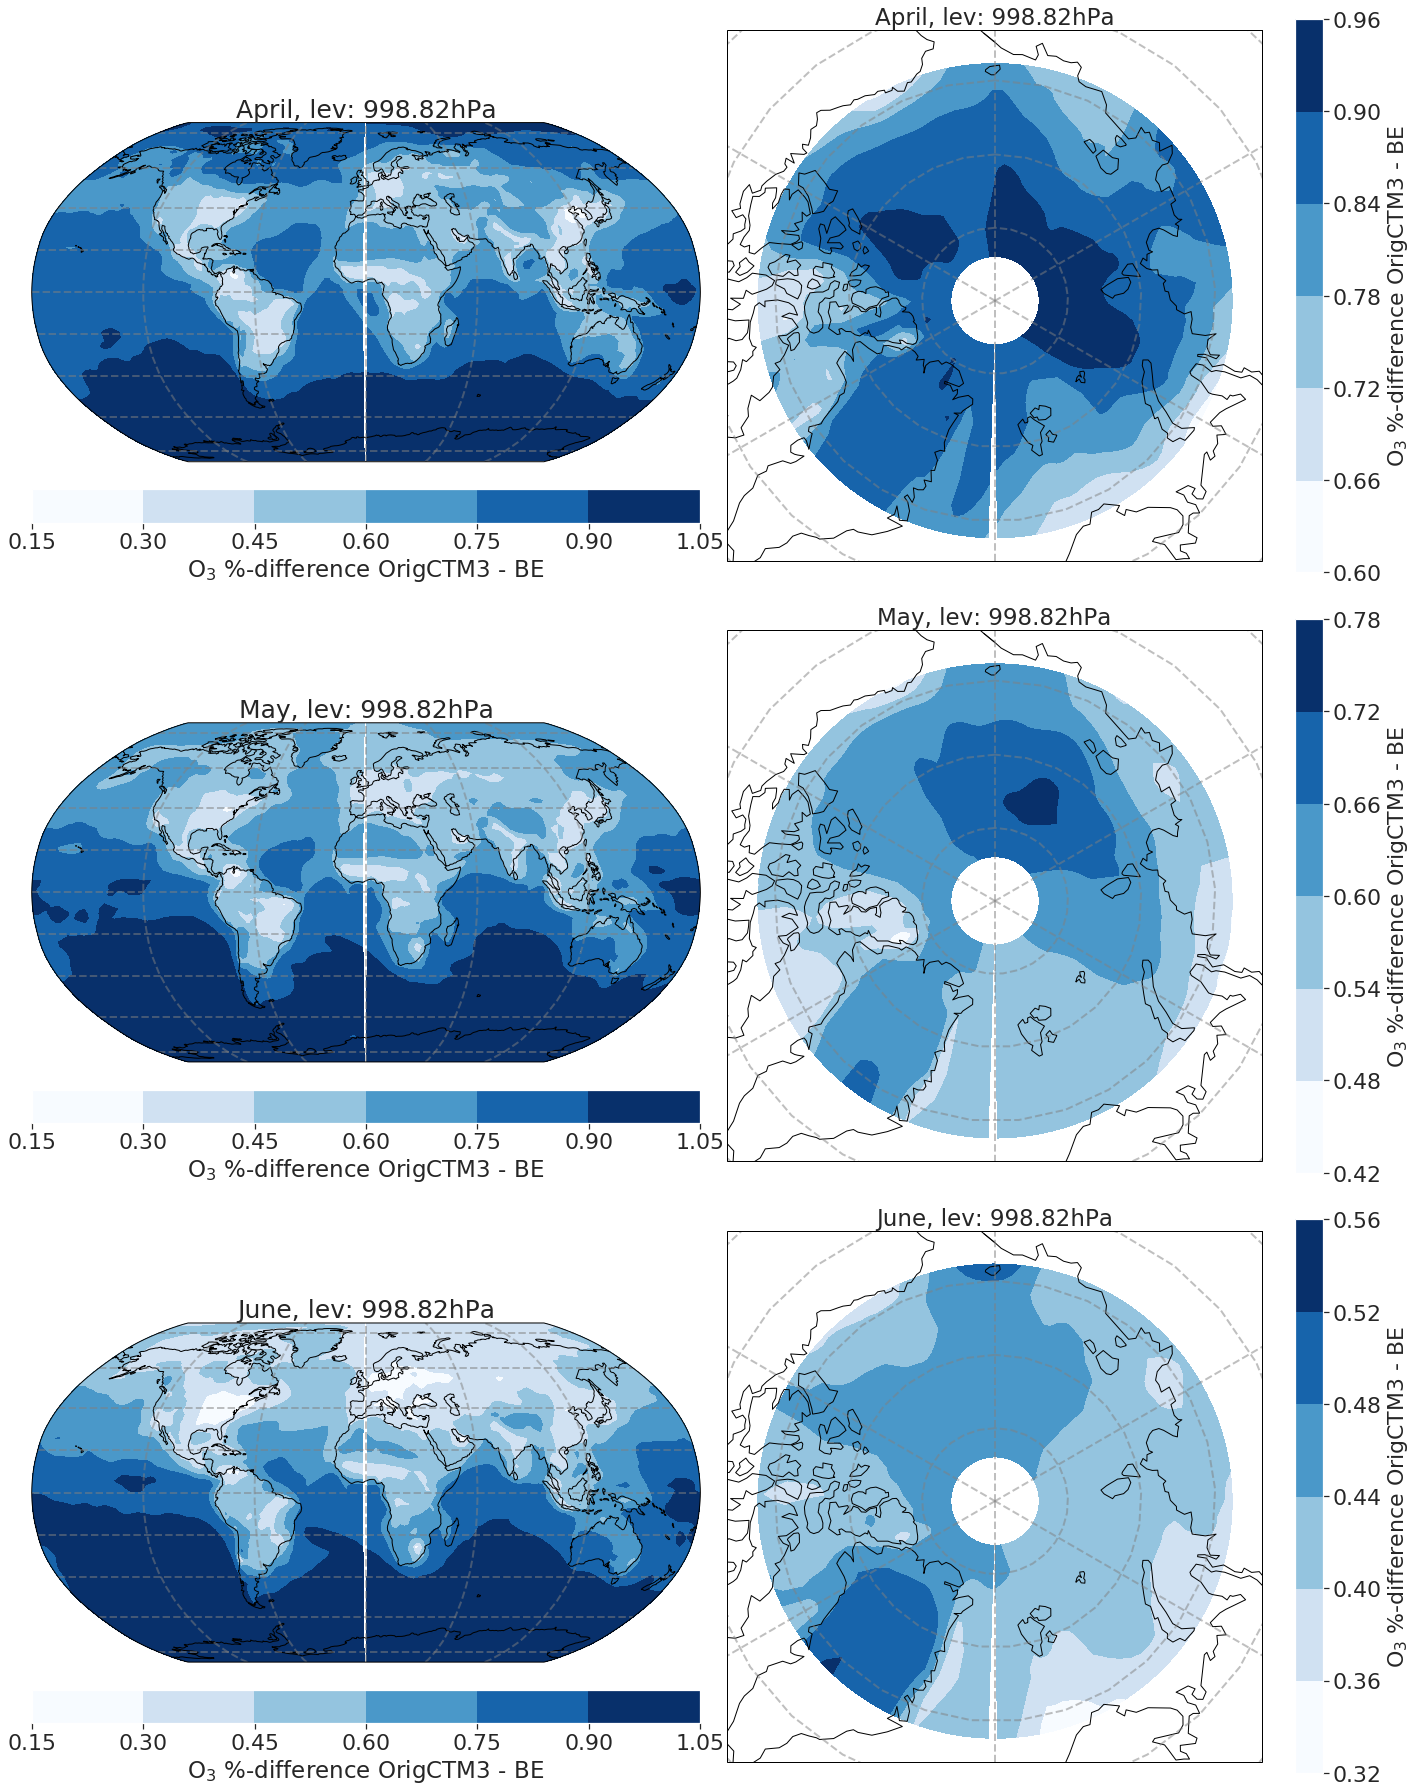
\includegraphics[width = \linewidth]{Chapter6_Results/images/Orig_BE_comp/BE_origPD_percent_lev0_AprJune_2001.png}
    \caption{Percentage difference in ozone monthly mean in the first model layer between the original CTM3 and the BE-branch globally (left columns) and in the Arctic (right columns) in the months April (top figures), May (middle figures) and June (bottom figures) in 2001 \textbf{Note:} the colorbar axis are not equal}
    \label{fig:BE_origPD_percent_AprJun}
\end{figure}

%%% SKAL TIL APPENDIX

\clearpage
\section{Radiative Forcing}\label{app:RF}

%%% SKAL TIL APPENDIX

\begin{figure}[ht]
    \centering
    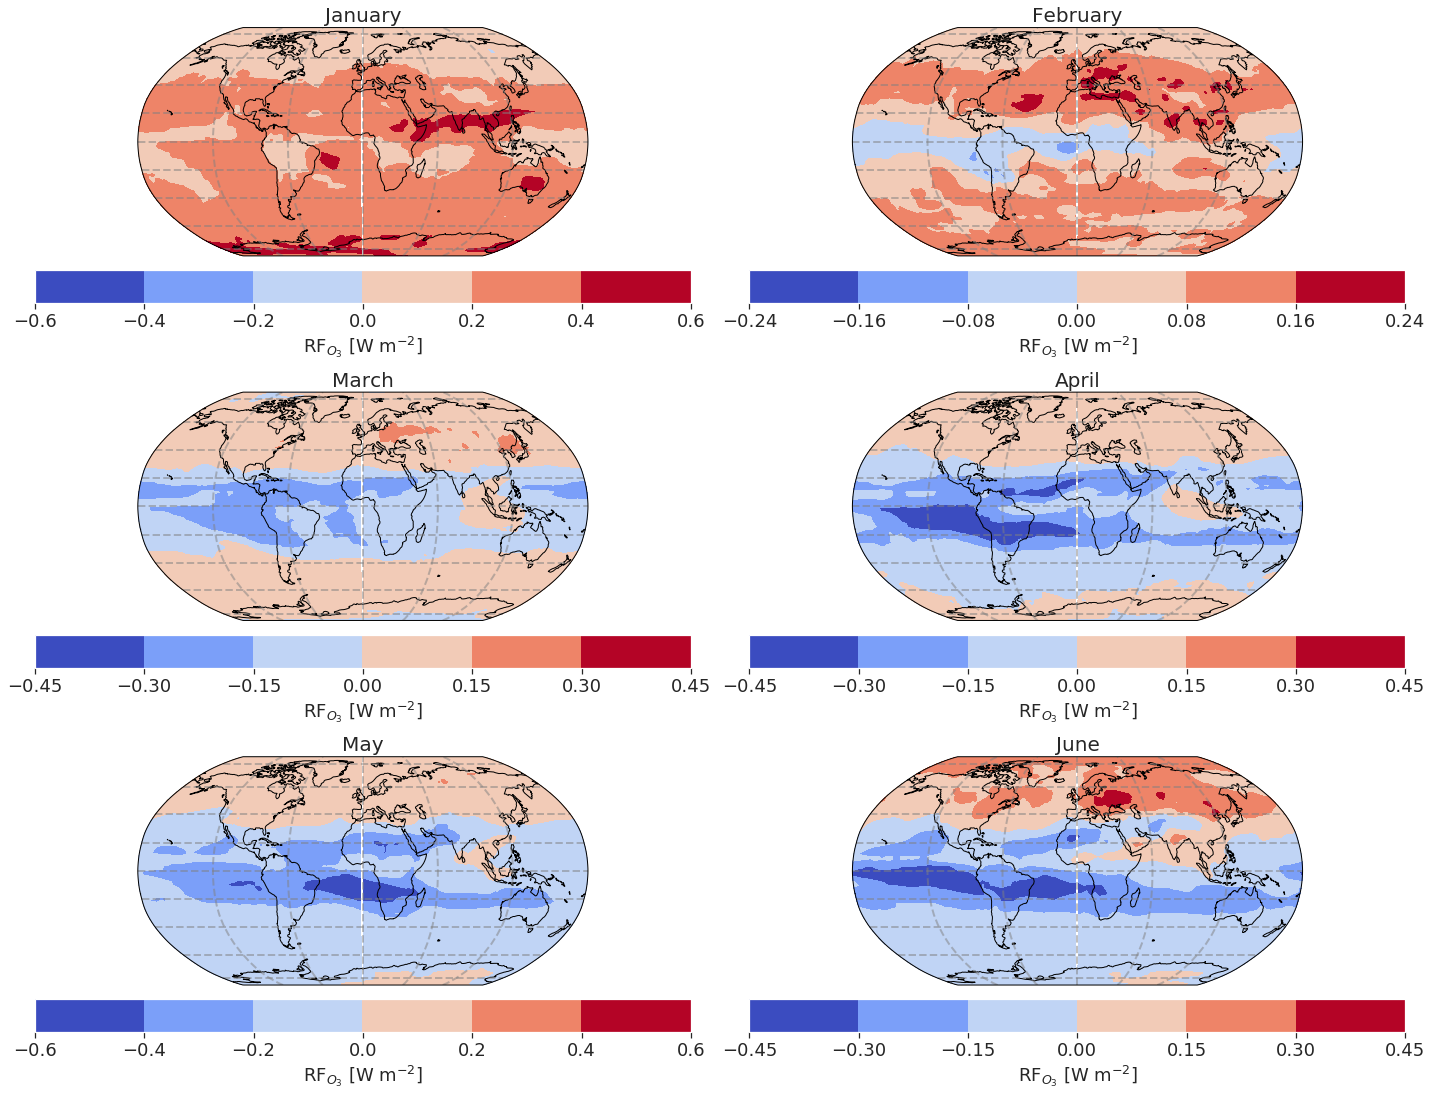
\includegraphics[width = \linewidth]{Chapter6_Results/images/RF/BE_RF_global_2001.png}
    \caption{Global RF-field (in Wm$^{-2}$) for the total tropospheric column up to the tropopause, produced using the BE-branch in 2001}
    \label{fig:BE_RF_global_2001}
\end{figure}

\begin{figure}[ht]
    \centering
    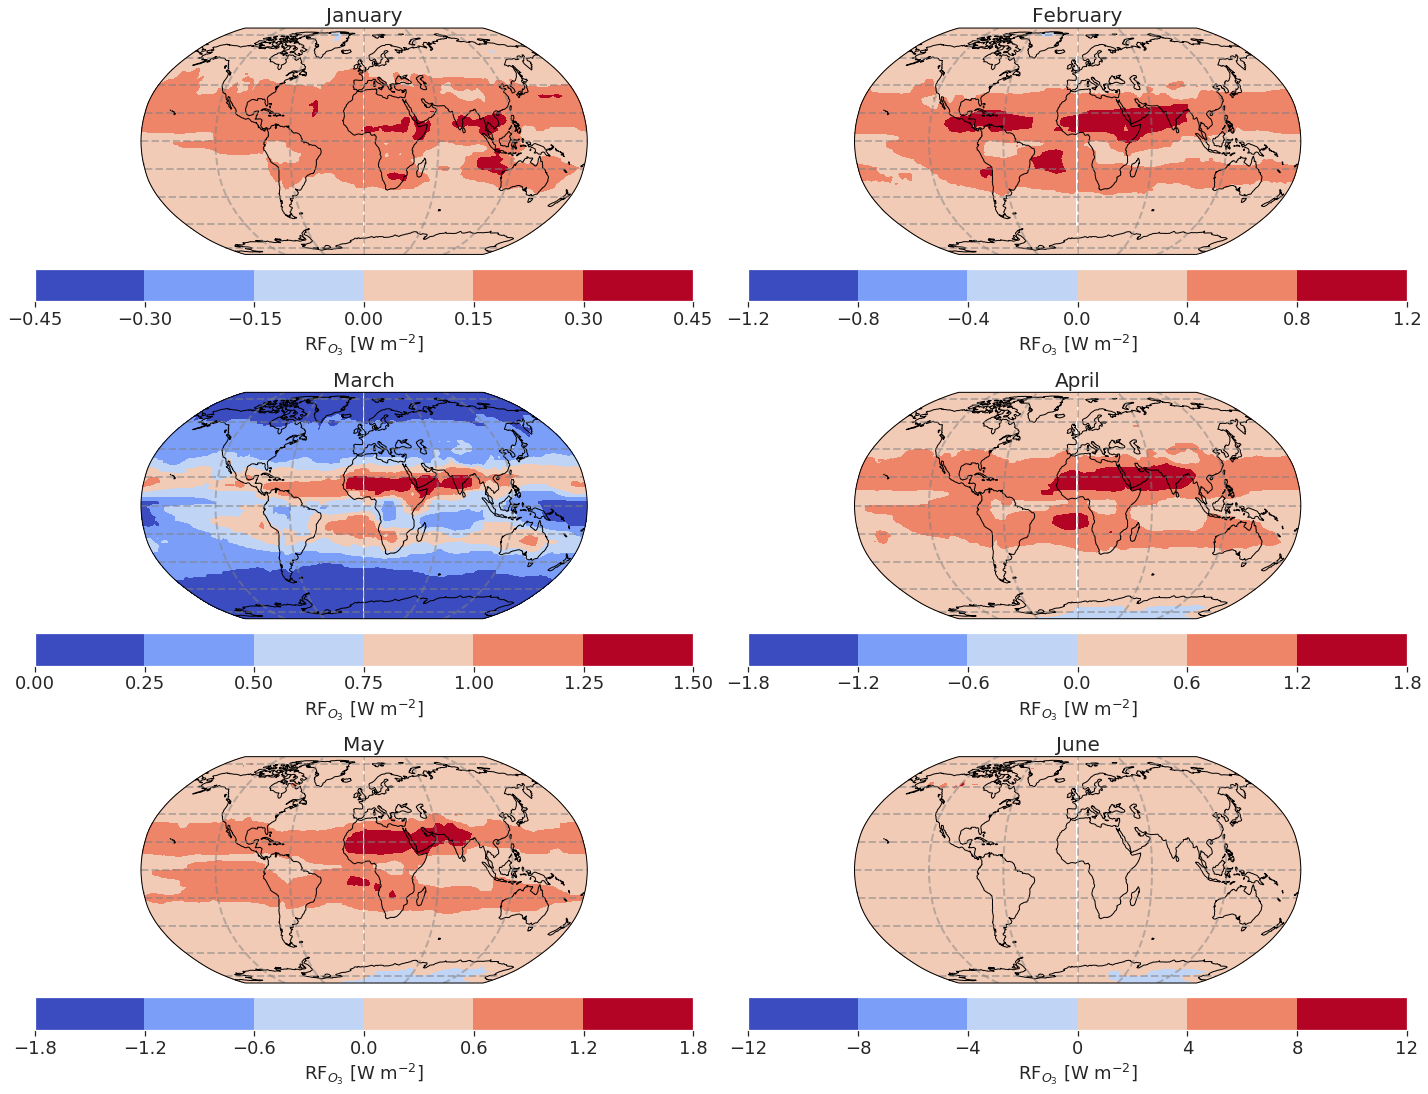
\includegraphics[width = \linewidth]{Chapter6_Results/images/RF/RF_USE/Appendix/BE_RF_global_2013.png}
    \caption{Global RF-field (in Wm$^{-2}$) for the total tropospheric column up to the tropopause, produced using the BE-branch in 2013}
    \label{fig:BE_RF_global_2013}
\end{figure}

\begin{figure}[ht]
    \centering
    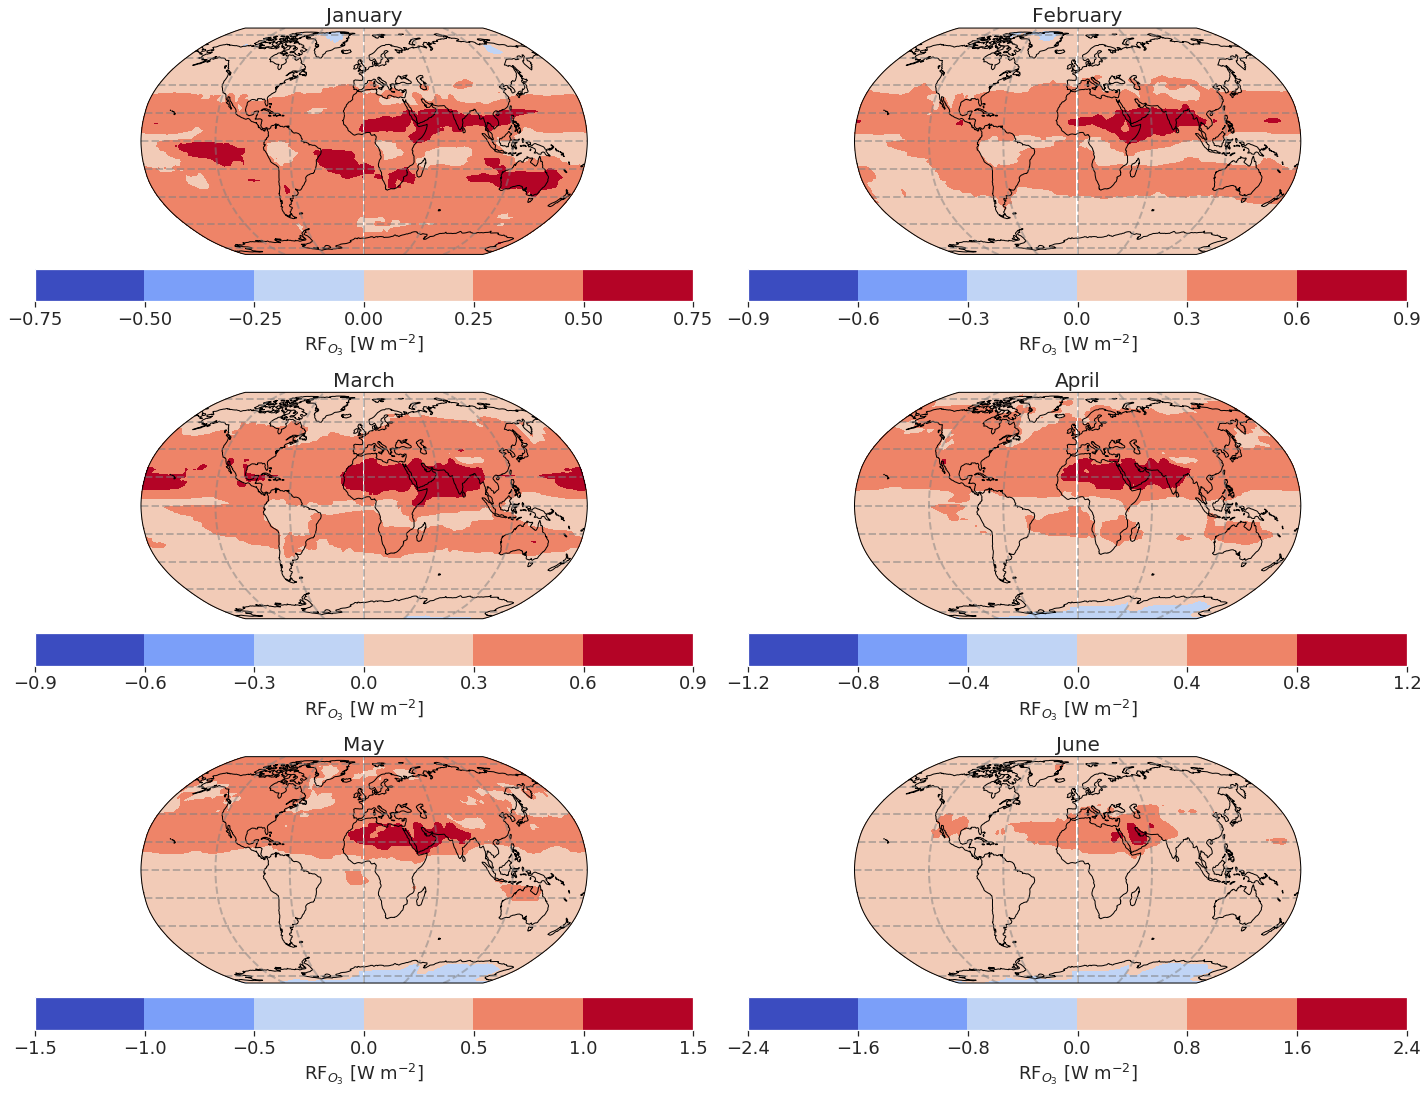
\includegraphics[width = \linewidth]{Chapter6_Results/images/RF/RF_USE/Appendix/Orig_RF_global_2001.png}
    \caption{Global RF-field (in Wm$^{-2}$) for the total tropospheric column up to the tropopause, produced using the Original CTM3 in 2001}
    \label{fig:orig_RF_global_2001}
\end{figure}
\begin{figure}[ht]
    \centering
    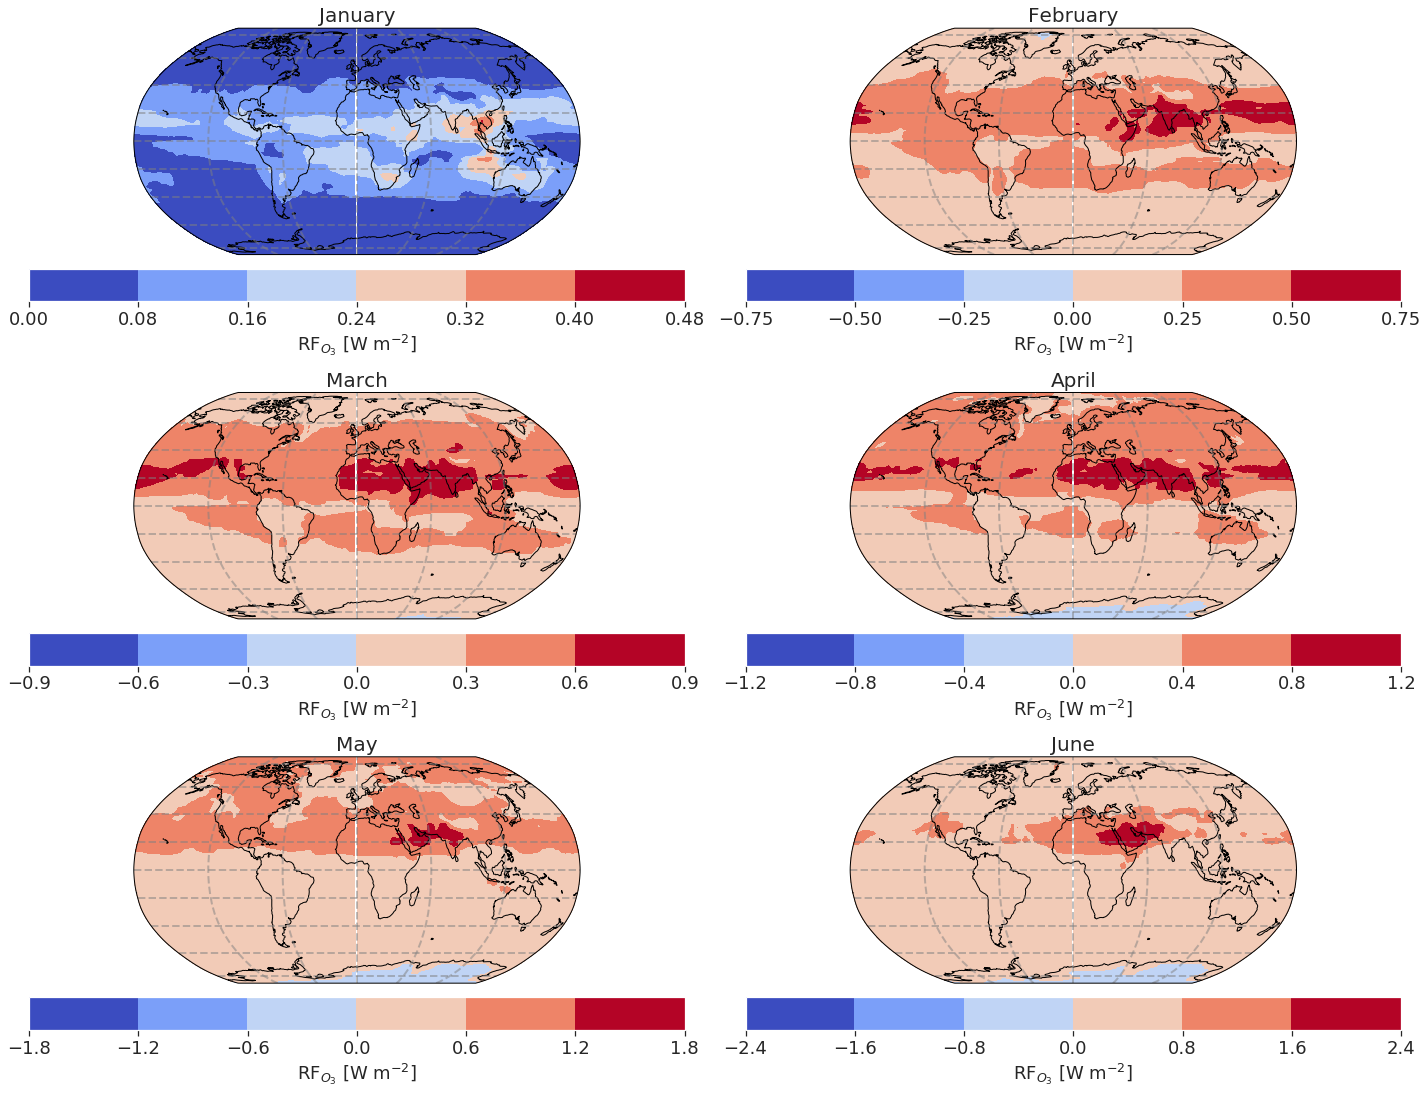
\includegraphics[width = \linewidth]{Chapter6_Results/images/RF/RF_USE/Appendix/Orig_RF_global_2013.png}
    \caption{Global RF-field (in Wm$^{-2}$) for the total tropospheric column up to the tropopause, produced using the Original CTM3 in 2013. \textbf{Note:} the colorbar axis are not equal}
    \label{fig:orig_RF_global_2013}
\end{figure}
